\clearpage{\pagestyle{empty}\cleardoublepage}

\chapter{The Tag Rate Function method}\label{app:trf}

When requiring high \btag ged jet multiplicity in an analysis, 
usually the available statistics in Monte Carlo simulated  samples 
is significantly reduced. This leads to large fluctuations
for the final discriminant variable distribution
and, as a direct consequence, reduced sensitivity of
the search because of unphysical variations of 
the systematic uncertainties affected by the unreliable
statistical uncertainties.
Furthermore this can introduce a bias in the observed limits
depending on the side of the fluctuation of the Monte Carlo
templates with respect to the data in the final signal region.
A Tag Rate Function (TRF) method can mitigate this problem
by keeping the full Monte Carlo pre-tag statistics and deriving
the shape and normalization predictions in the \btag ged channels
through a reweighting procedure.

While the vector-like signal samples, obtained using a fast simulation
of the detector, have enough statistics in the final channels for
both the \wbx\ and \htx\ analyses, Monte Carlo backgrounds are highly
affected by the cuts specifically designed to reduce their presence
in the final selection.
Therefore, the TRF method is applied to all Monte Carlo samples in
the \htx\ analysis, which requires high \btag ged jet multiplicities
in its search channels, and to all non-\ttbar\ Monte Carlo samples
($W$+jets, $Z$+jets, diboson, single-top, $\ttbar V$) in the \wbx\ 
analysis, which requires only one \btag ged jet but drastically
reduces the background contribution to the signal region through
tight selection requirements.

In this appendix the principle of this method and the various 
studies performed to validate its usage in the analyses
are discussed.



\section{TRF method principle}

When a direct cut on the
\btag ging weight returned by the \btag ging algorithm
is applied, events that do not have the requested number
of jets satisfying this cut are rejected. Considering that
commonly chosen working points for the \btag ging algorithms
have a measured efficiency of 70\%, it is easy to imagine the
potential loss in acceptance when requiring more that one
\btag ged jets.
By using the TRF method, no event is rejected based on 
the $b$-tagged jet multiplicity, but instead all the pre-tag events 
are reweighted.
The event weight is calculated using the
per-jet  \btag ging efficiency
(which depends on the jet's $\pt$, $\eta$ and true jet flavour)
and based on the kinematics and flavour of the 
jets found in each event.
This weight can be interpreted as the probability of the 
given event to contain the desired number of \btag ged jets. 

Given a jet with $\pt$, $\eta$ and flavour $f$, its 
tagging probability can be written as:
\begin{equation}
	\varepsilon \left(\pt,|\eta|,f\right).
\end{equation}

For instance, for a given event with $N$ jets, the probability of 
containing exactly one $b$-tagged jet can be computed as:
\begin{align}
	P_{=1} &= \sum\limits_{i=1}^N \left( \varepsilon_{i} \prod\limits_{j \neq i} \left( 1 - \varepsilon_{j} \right) \right).\end{align}
This can be generalized as the probability of containing exactly $M$
$b$-tagged jets by iterating over all the possible subsets of $M$ and $N-M$
jets as:
\begin{align}
        P_{=M} &= \sum\limits_{i,\dots,m=1}^N 
        \left( 
        \prod\limits_{i=1}^{m=M} \varepsilon_{i}  
        \prod\limits_{j=m+1}^N \left( 1 - \varepsilon_{j} \right) 
        \right),
	%P_{=m} &= \sum\limits_{i,j,\dots,m=1}^N \left( \varepsilon_{i}\varepsilon_{j}\dots\varepsilon_{m}(1-\delta(i,j,\dots,m)) \prod\limits_{k \neq i\neq j \dots\neq m} \left( 1 - \varepsilon_{k} \right) \right), \\
\end{align}
and in general the probability for inclusive $b$-tagging selections can be
computed:
\begin{align}
	P_{=0} &= \prod\limits_{i=1}^N \left( 1 - \varepsilon_{j} \right), \\
	P_{\geq 1} &= 1 - P_{=0},\\
&\dots \notag\\
	P_{\geq m} &= 1 - \sum\limits_{i=0}^{m-1} P_{=i}.
\end{align}

\subsection{Validation}
This method relies on the correct calibration of the \btag ging efficiency in 
Monte Carlo samples. 
Closure tests performed with the official calibration files have shown that 
the efficiency parametrization is not as accurate as expected.
Assuming a correct calibration, the average of the histogram of 
$1/\varepsilon$ vs $\eta$, $\pt$ and true jet flavour should be 
flat and with mean equal to one.

In Figure~\ref{fig:closure} the result of this test is shown, and it 
can be observed that for the official maps (the left colums) there 
are departures from closure of to up to 40\% in some regions of the light flavor
map, and on average of 13\%.
New efficiency maps have been derived using a combination 
of $t\bar{t}$ \texttt{MC@NLO}, $t\bar{t}$ \texttt{ALPGEN}, and 
\texttt{Protos} $\TT$ Monte Carlo samples.
The plots on the right column of Figure~\ref{fig:closure} 
show reasonably good closure for the newly derived efficiency map,
which will therefore be used for the probability computations in the TRF method.

\begin{figure}[h!tb]\begin{center}
	\subfigure[]{
    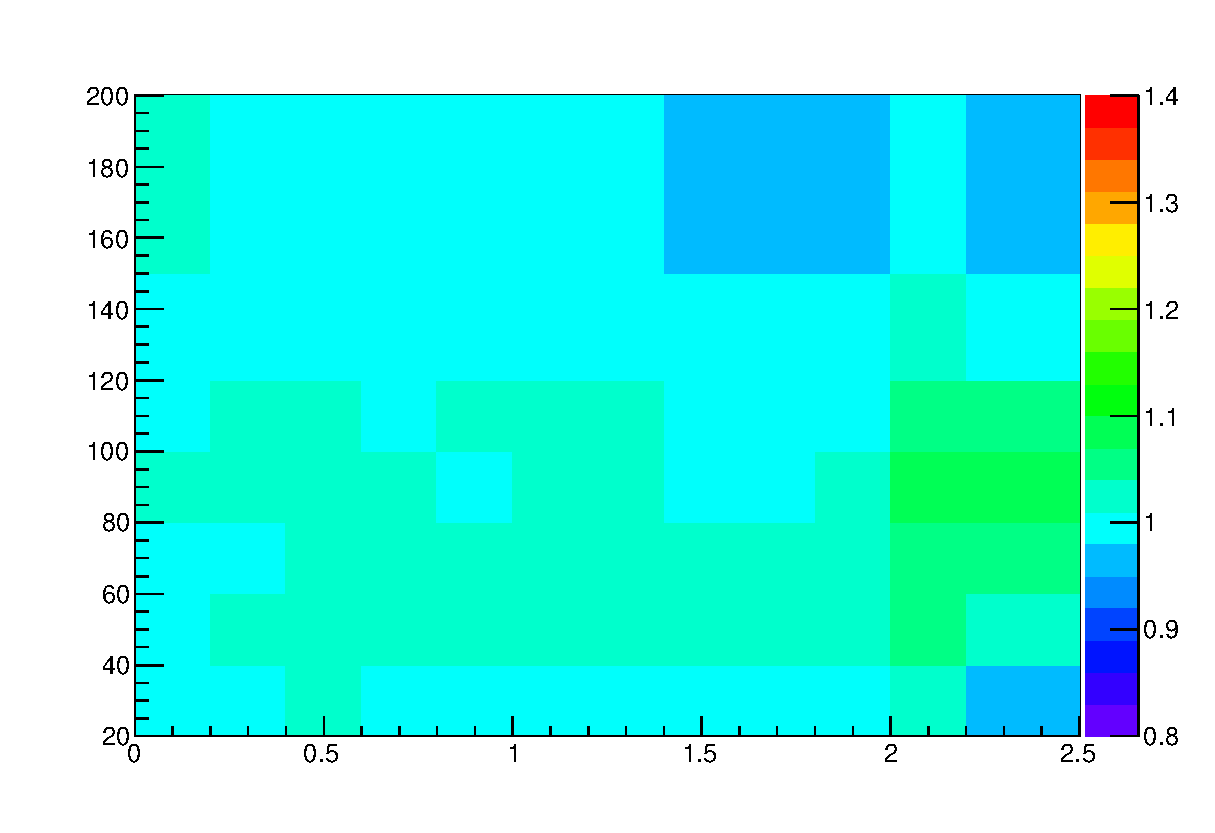
\includegraphics[width=0.45\textwidth]{appendices/figures/trf/5closureRebin.eps}}
	\subfigure[]{
    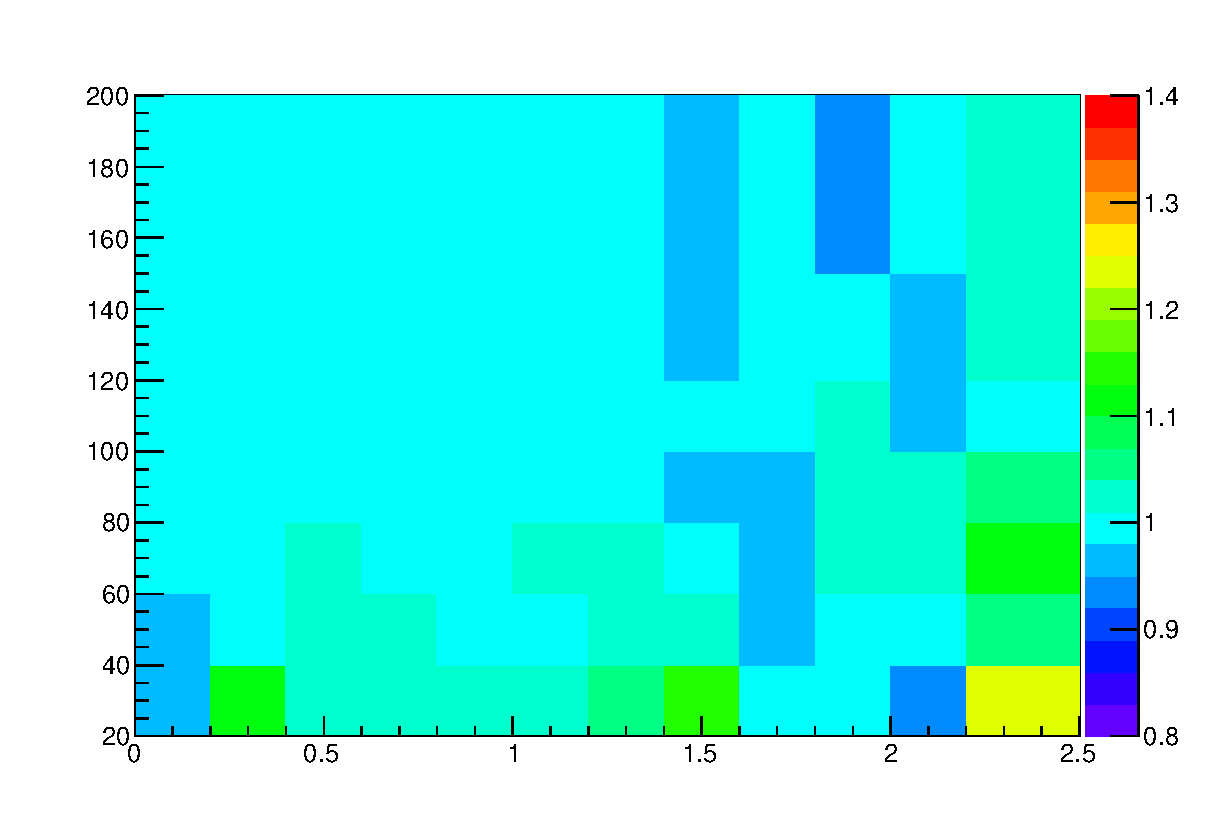
\includegraphics[width=0.45\textwidth]{appendices/figures/trf/5myclosureRebin.eps}}
	\subfigure[]{
    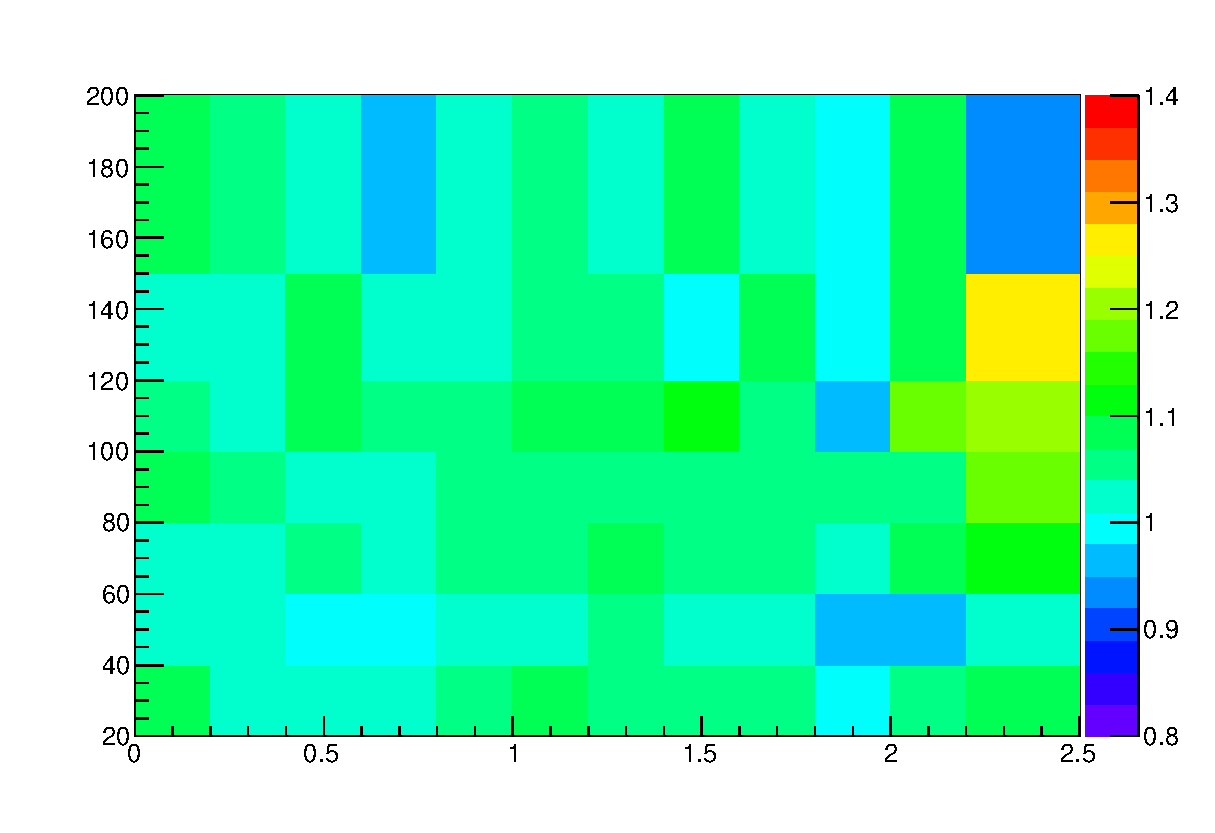
\includegraphics[width=0.45\textwidth]{appendices/figures/trf/4closureRebin.eps}}
	\subfigure[]{
    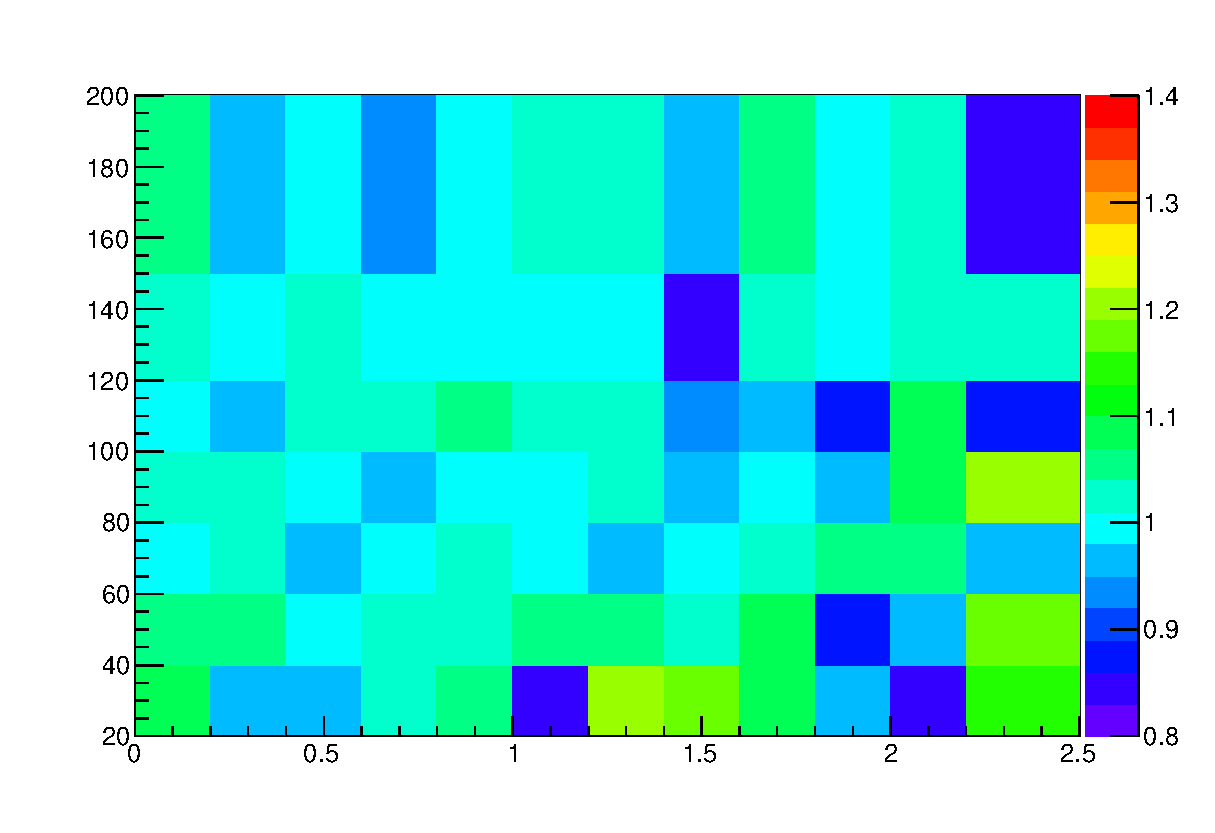
\includegraphics[width=0.45\textwidth]{appendices/figures/trf/4myclosureRebin.eps}}
	\subfigure[]{
    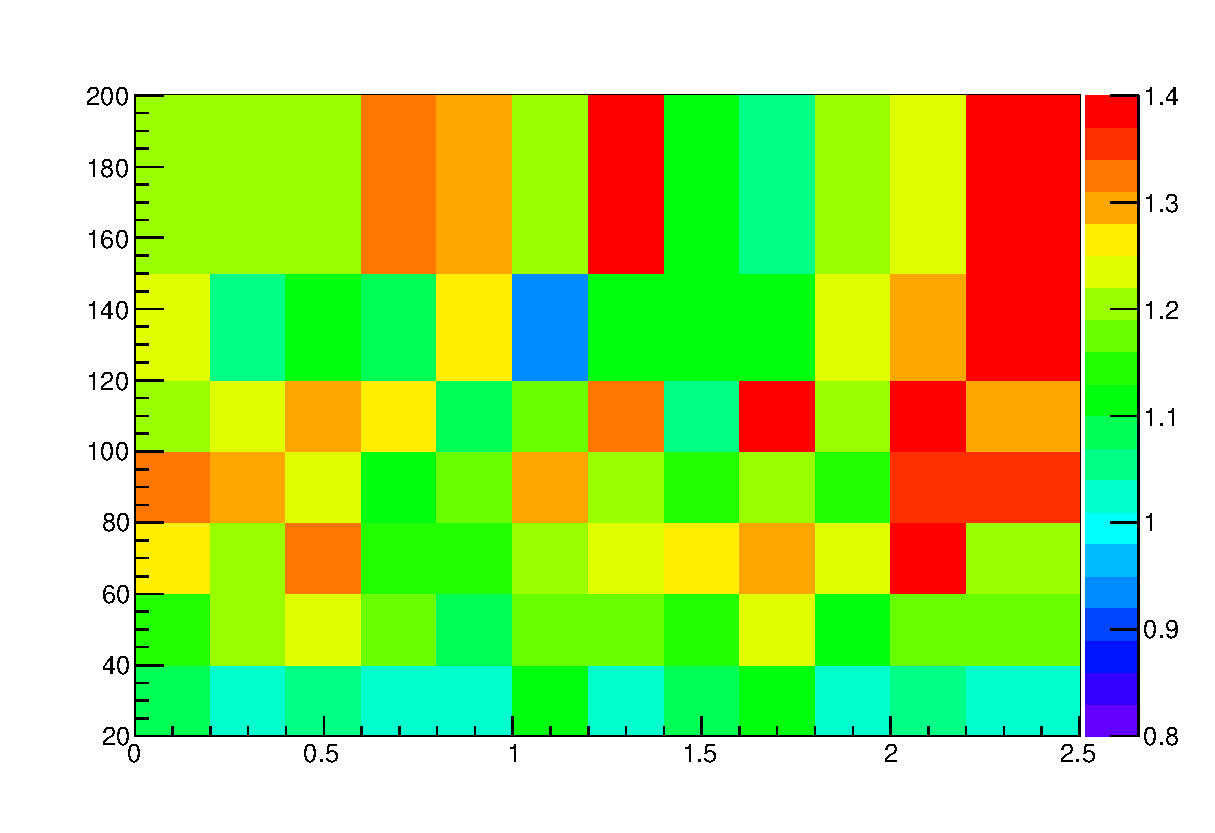
\includegraphics[width=0.45\textwidth]{appendices/figures/trf/0closureRebin.eps}}
	\subfigure[]{
    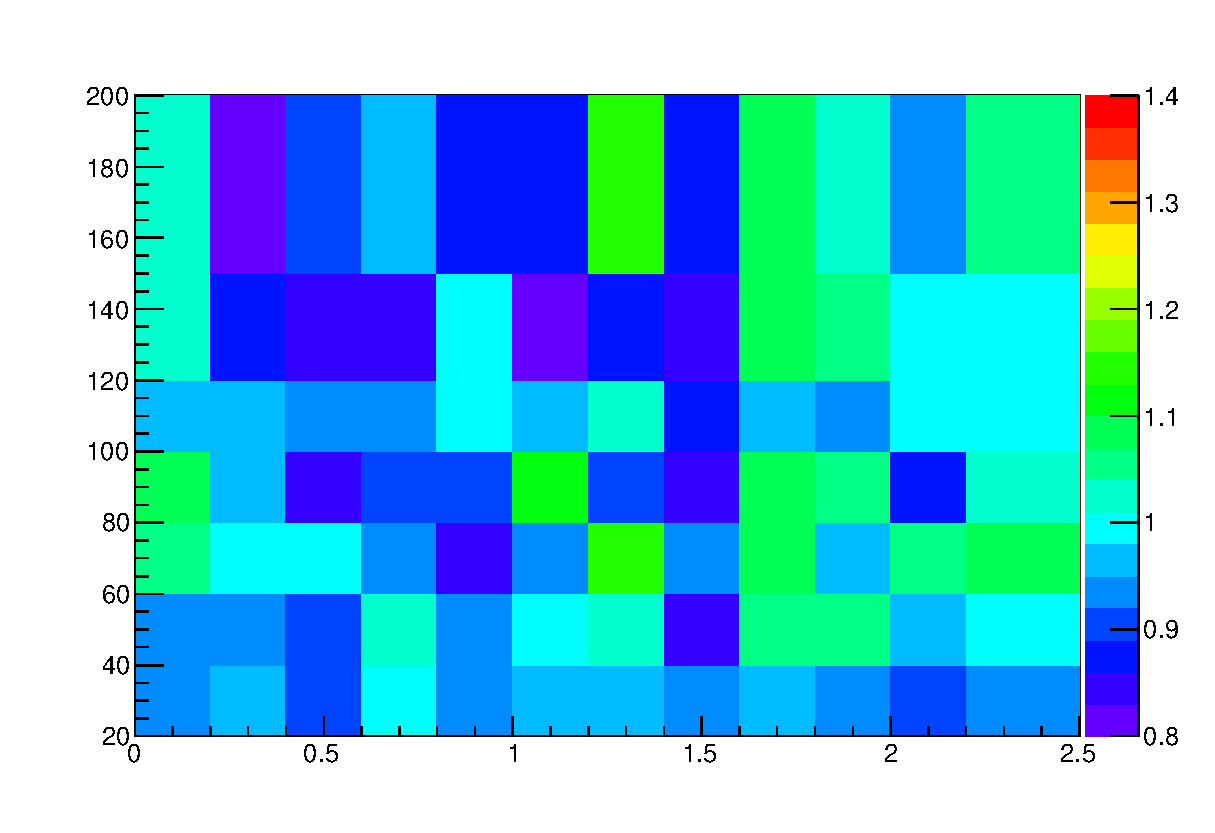
\includegraphics[width=0.45\textwidth]{appendices/figures/trf/0myclosureRebin.eps}}
	\caption{Results of the closure test using efficiency from the official calibration file (left column) and the private efficiency map (right column). The test is split in the different jet flavours: $b$-jets (top), $c$-jets (middle) and light jets (bottom).\label{fig:closure}}
\end{center}\end{figure}

As a validation check, Figure~\ref{fig:btags} compares the spectrum
of the number of \btag ged jets distribution in the  $t\bar{t}$ Monte Carlo
sample simulated with \texttt{ALPGEN} obtained using the TRF method
and the direct \btag ging. The shapes are found to be compatible.

\begin{figure}[h!tb]\begin{center}
	\subfigure[]{\label{fig:trf4j}
    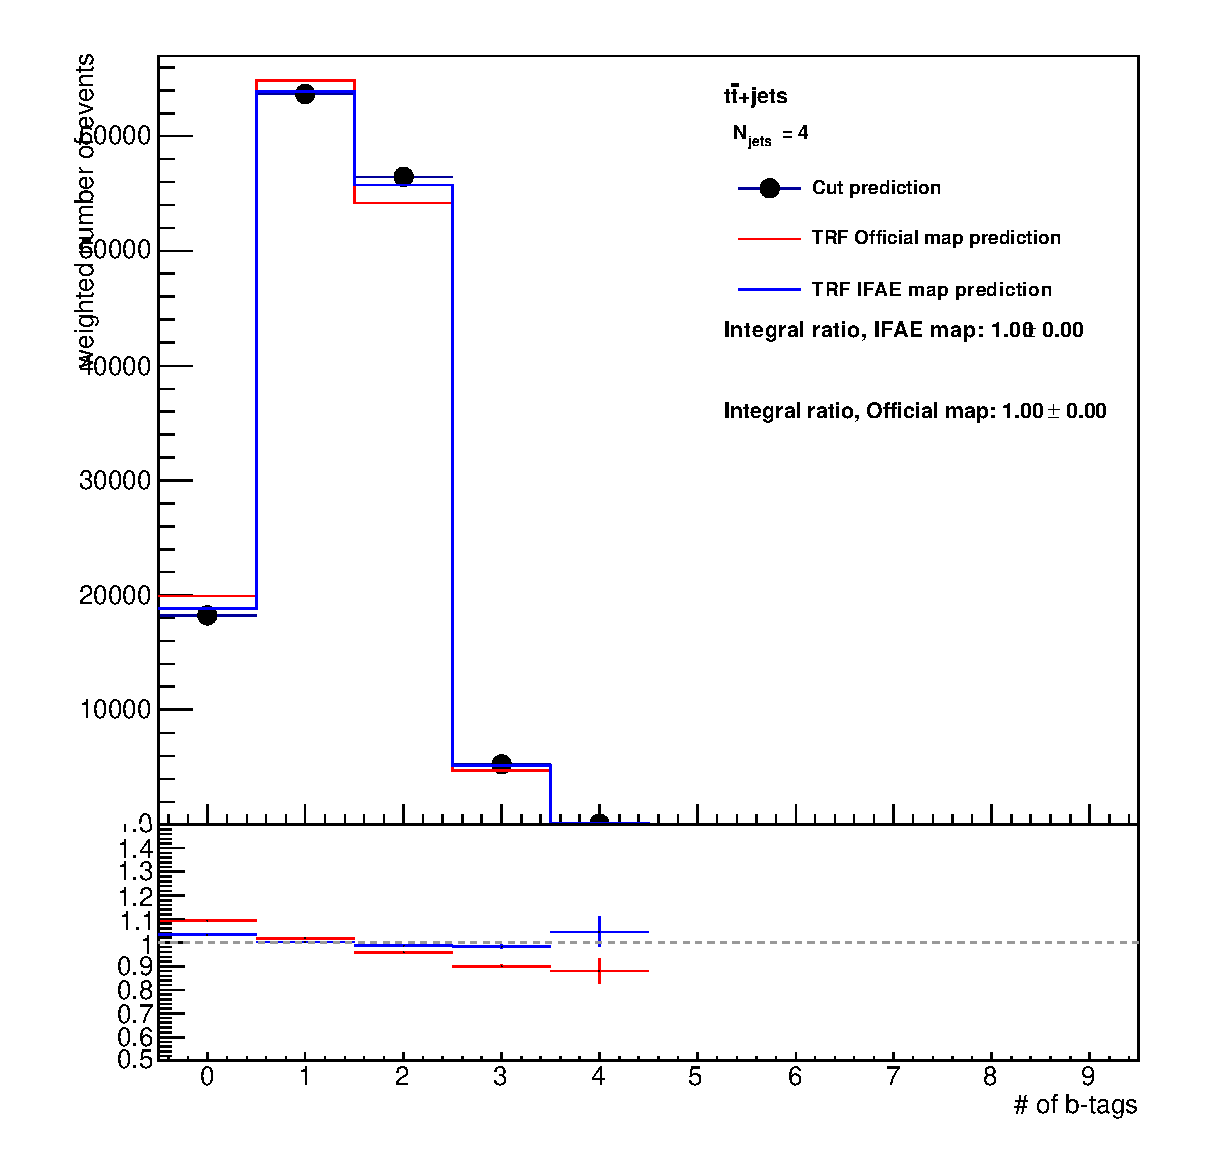
\includegraphics[width=0.32\textwidth]{appendices/figures/trf/ttbarAlpgen_HFOR_ntags_4jetex.eps}}
	\subfigure[]{\label{fig:trf5j}
    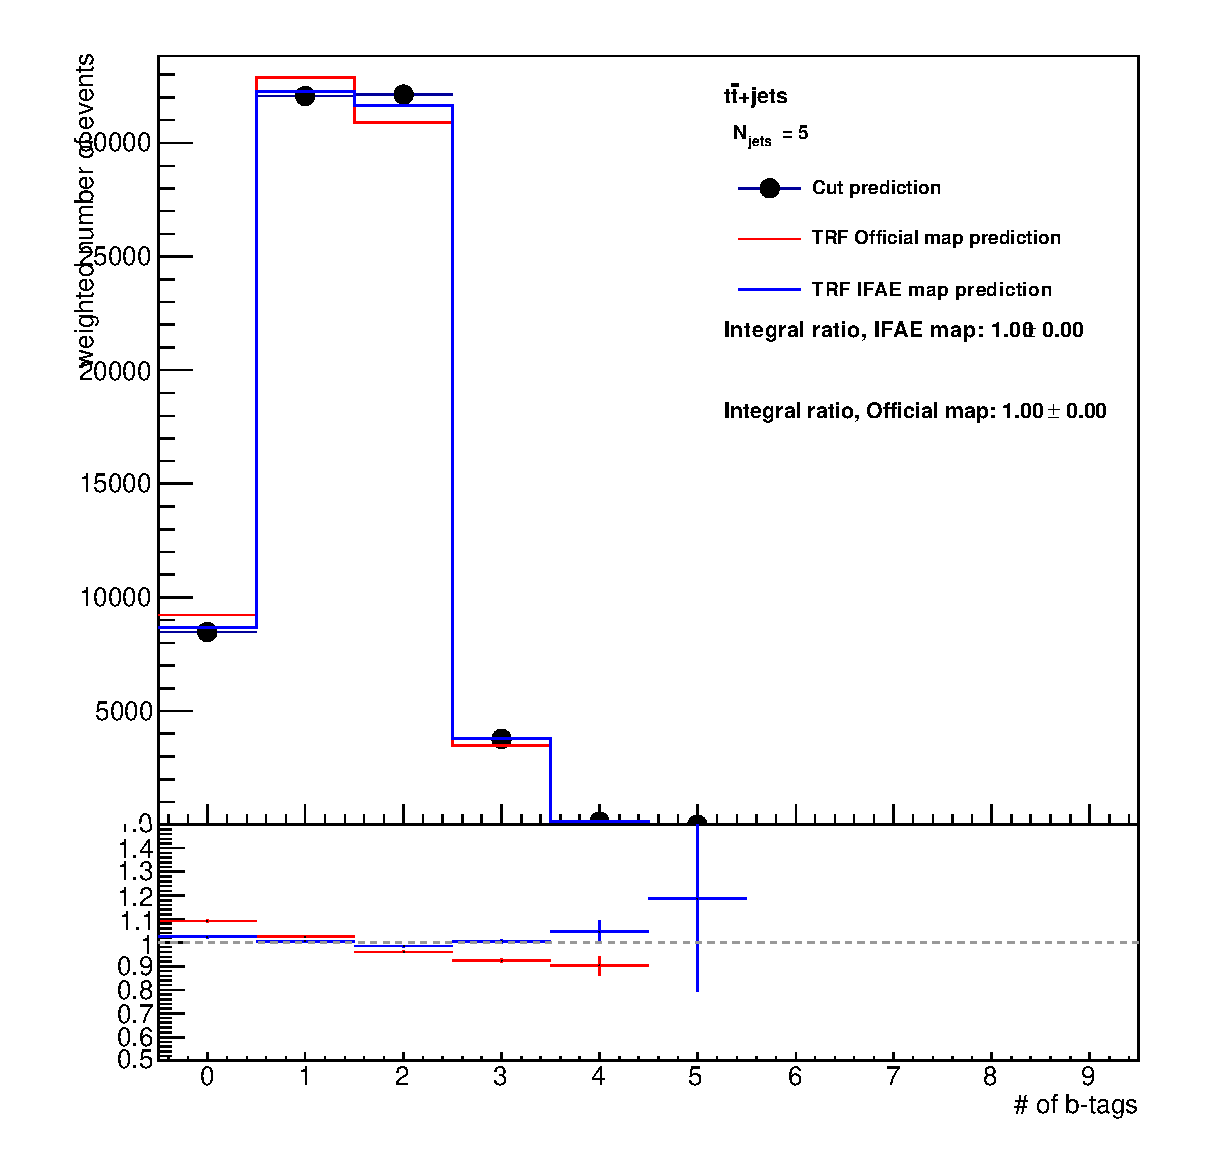
\includegraphics[width=0.32\textwidth]{appendices/figures/trf/ttbarAlpgen_HFOR_ntags_5jetex.eps}}
	\subfigure[]{\label{fig:trf6j}
    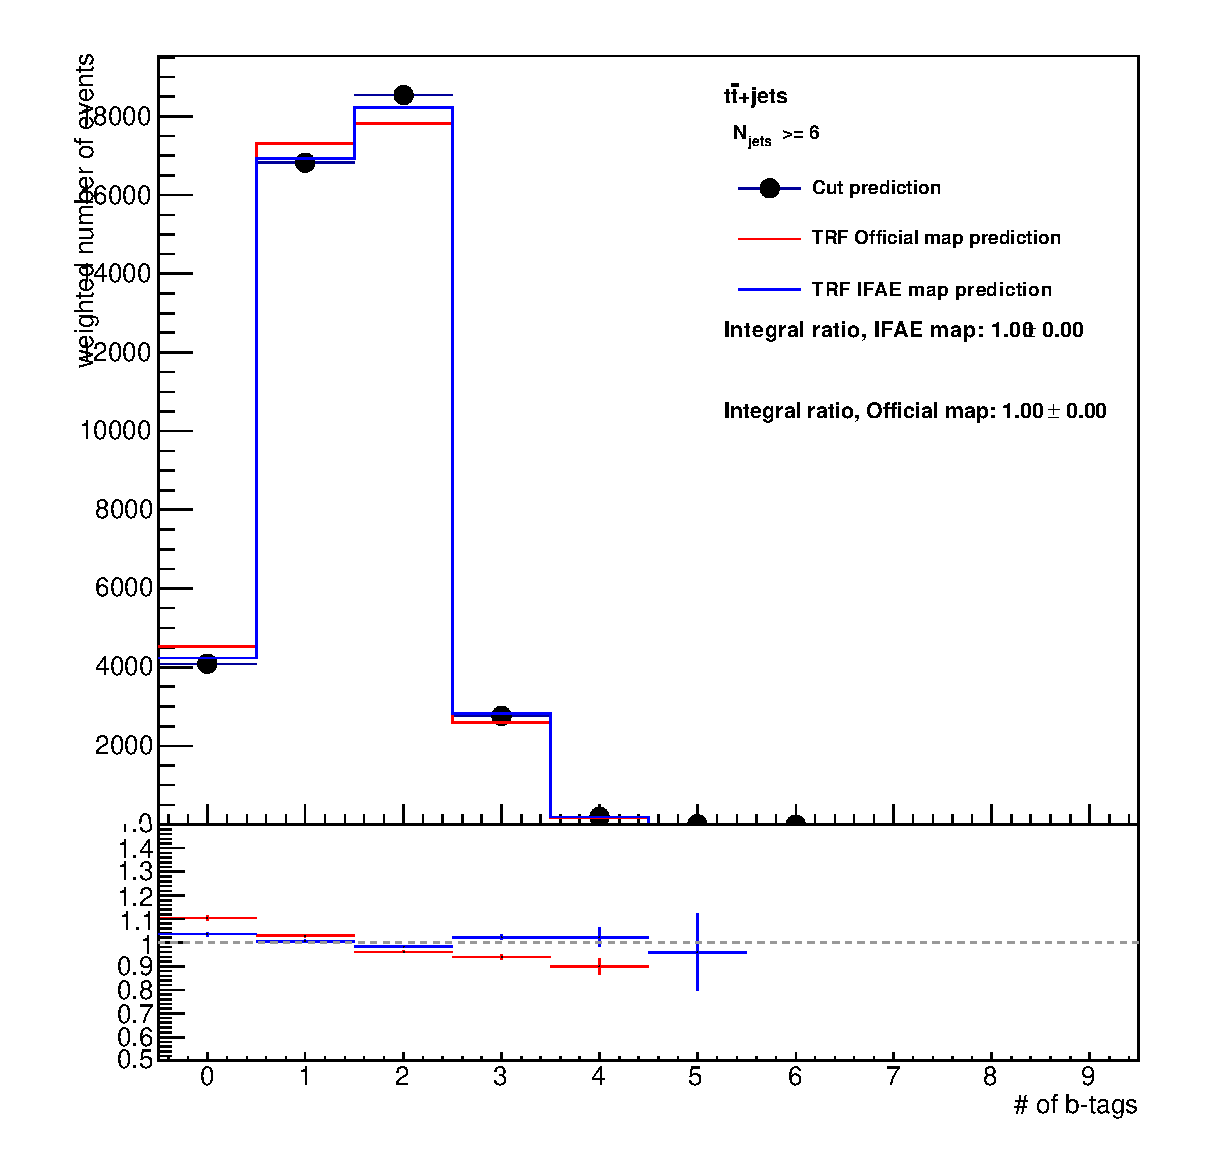
\includegraphics[width=0.32\textwidth]{appendices/figures/trf/ttbarAlpgen_HFOR_ntags_6jetin.eps}}
	\caption{Comparison of the TRF and direct $b$-tag cut prediction for the $b$-tag spectrum, in the 4 jet exclusive (a), 5 jet exclusive (b) and 6 jet inclusive (c) channels.\label{fig:btags}}
\end{center}\end{figure}


\section{TRF in the \wbx\ analysis}
%\section{TRF and \nontt\ background in the \wbx\ analysis}

As previously mentioned, the \wbx\ analysis applies the
TRF method only to Monte Carlo simulated samples of
$W/Z$+jets, single top, diboson and $t\bar{t}V$.
Table~\ref{tab:TRFvsCUT} compares the predicted yields 
at the various steps of the selection obtained
applying the TRF method and the direct cut on the
\btag ging weight for each of these simulated
processes. It can be seen that good agreement
is observed for selections where the direct \btag ging
still leaves sufficient Monte Carlo statistics,
while going tighter into the signal regions only
the TRF method returns non-zero prediction.
Also to be noted is that in all cases
the statistical uncertainty on the predicted yield is
improved by the TRF method.


\section{TRF in the \htx\ analysis}

The TRF method is used for all the Monte Carlo backgrounds in the
\htx\ analysis due to the high \btag\ multiplicity
(up to $\geq 4$) required. The validity of the method is checked by comparing 
the normalization and shape of final discriminant $H_T$ distribution
for the most relevant background, the \ttbar\ sample simulated with
\texttt{ALPGEN}, in different jet and \bjet multiplicity channels,
using the TRF method and direct \btag ging.
As it can be seen in these plots, the prediction obtained with the TRF 
method is accurate up to the statistical error.


\begin{landscape}
\begin{figure}[htb]\begin{center}
\vskip-.5cm
\hskip-1cm
\resizebox{1.5\textwidth}{!}{
	\subfigure[]{
  	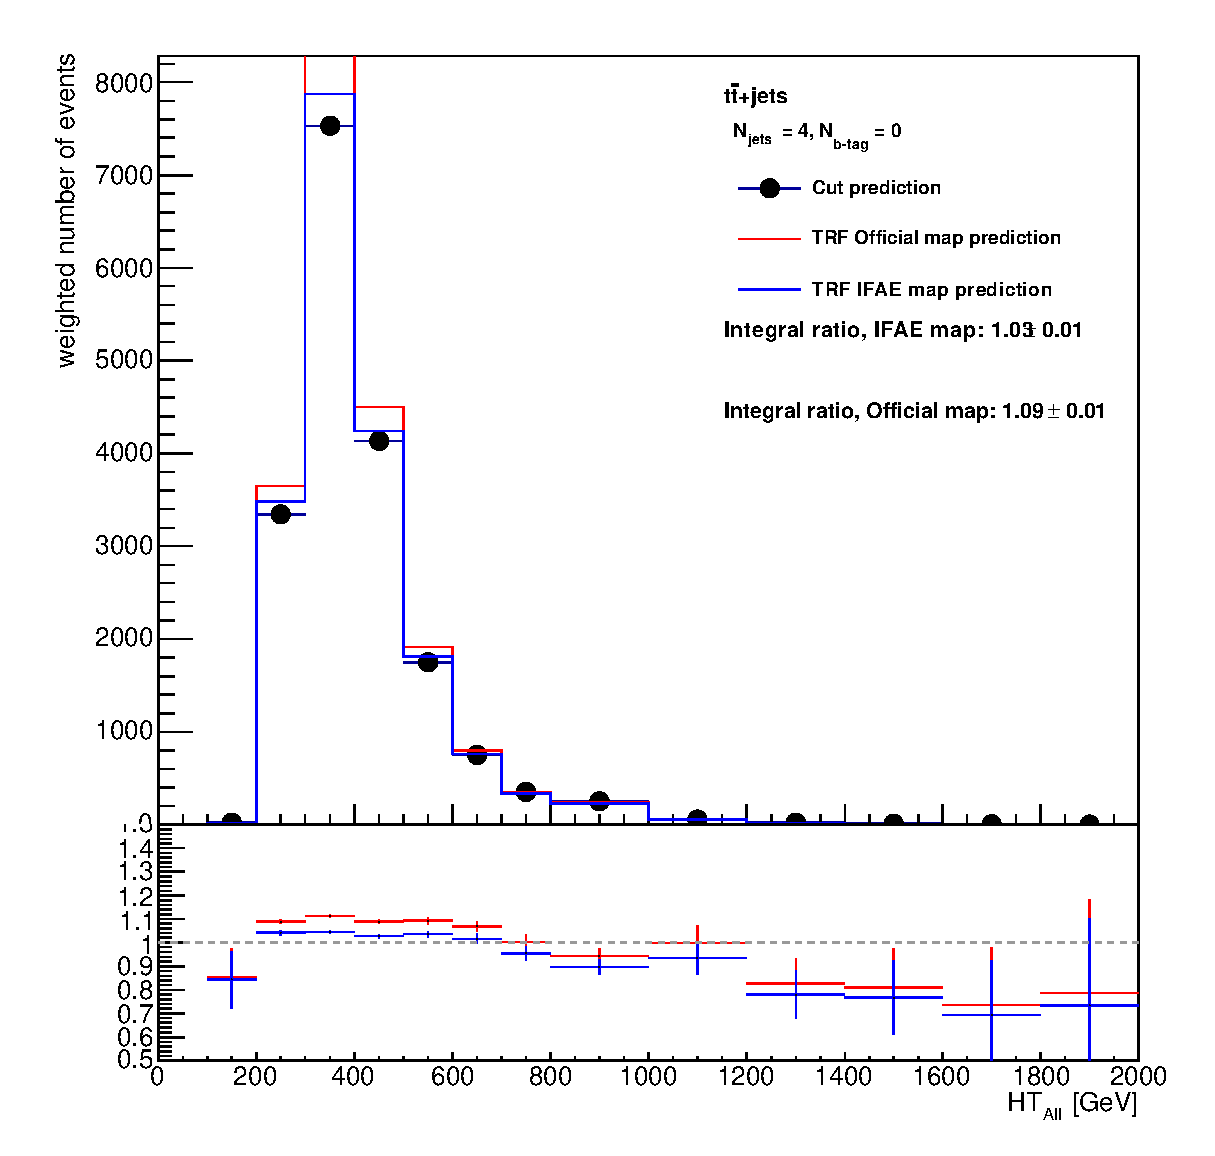
\includegraphics[width=0.3\textwidth]{appendices/figures/trf/ttbarAlpgen_HFOR_htall_4jetex0btagex.eps}}
	\subfigure[]{
  	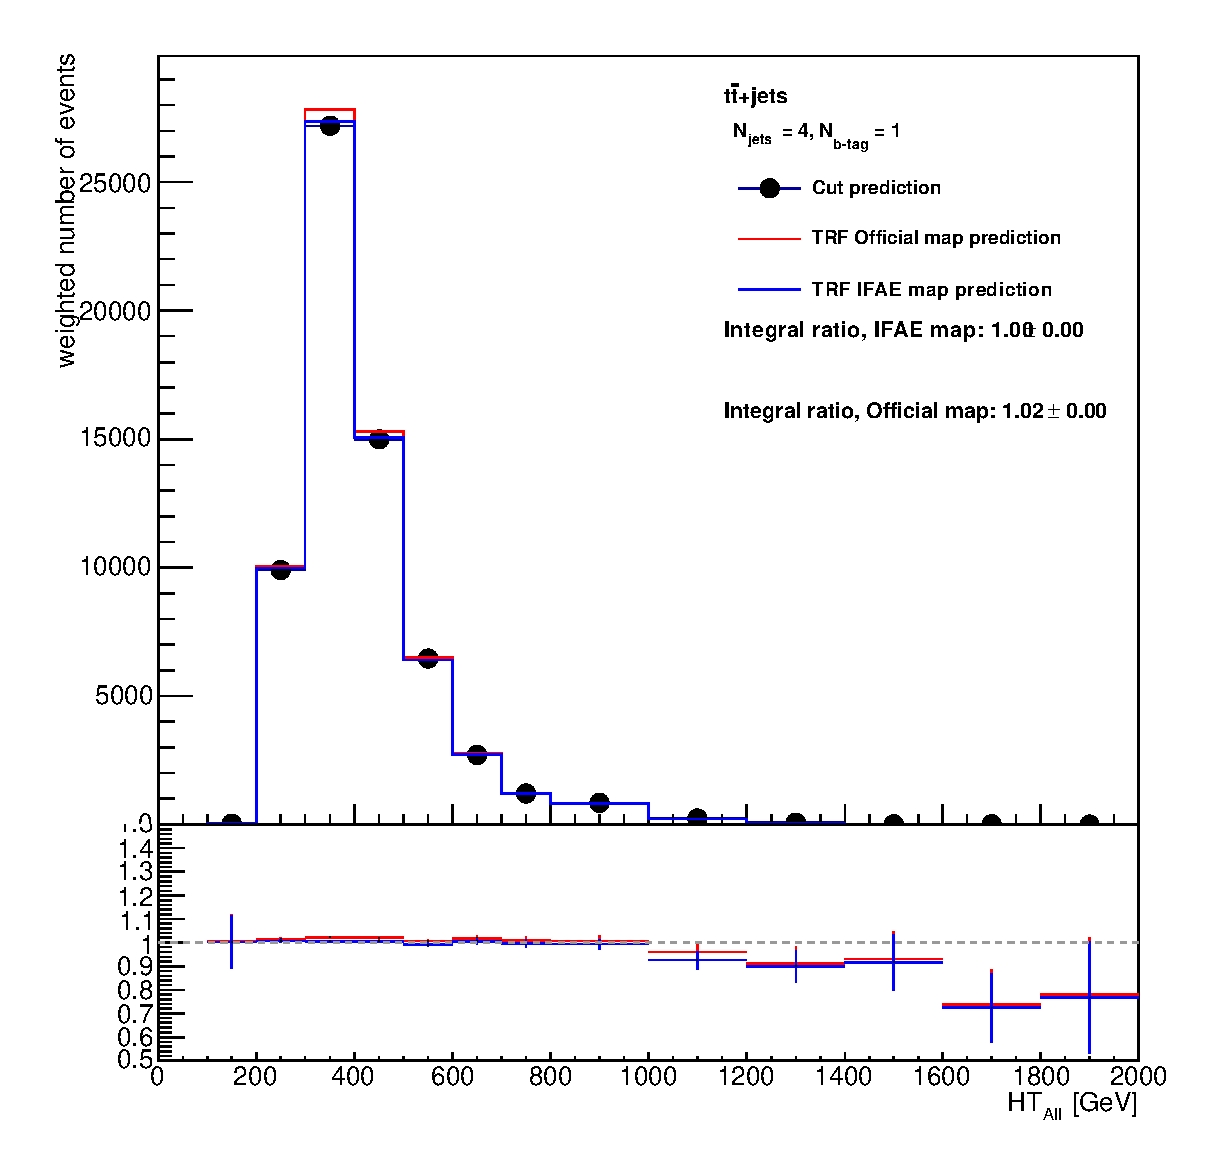
\includegraphics[width=0.3\textwidth]{appendices/figures/trf/ttbarAlpgen_HFOR_htall_4jetex1btagex.eps}}
	\subfigure[]{
  	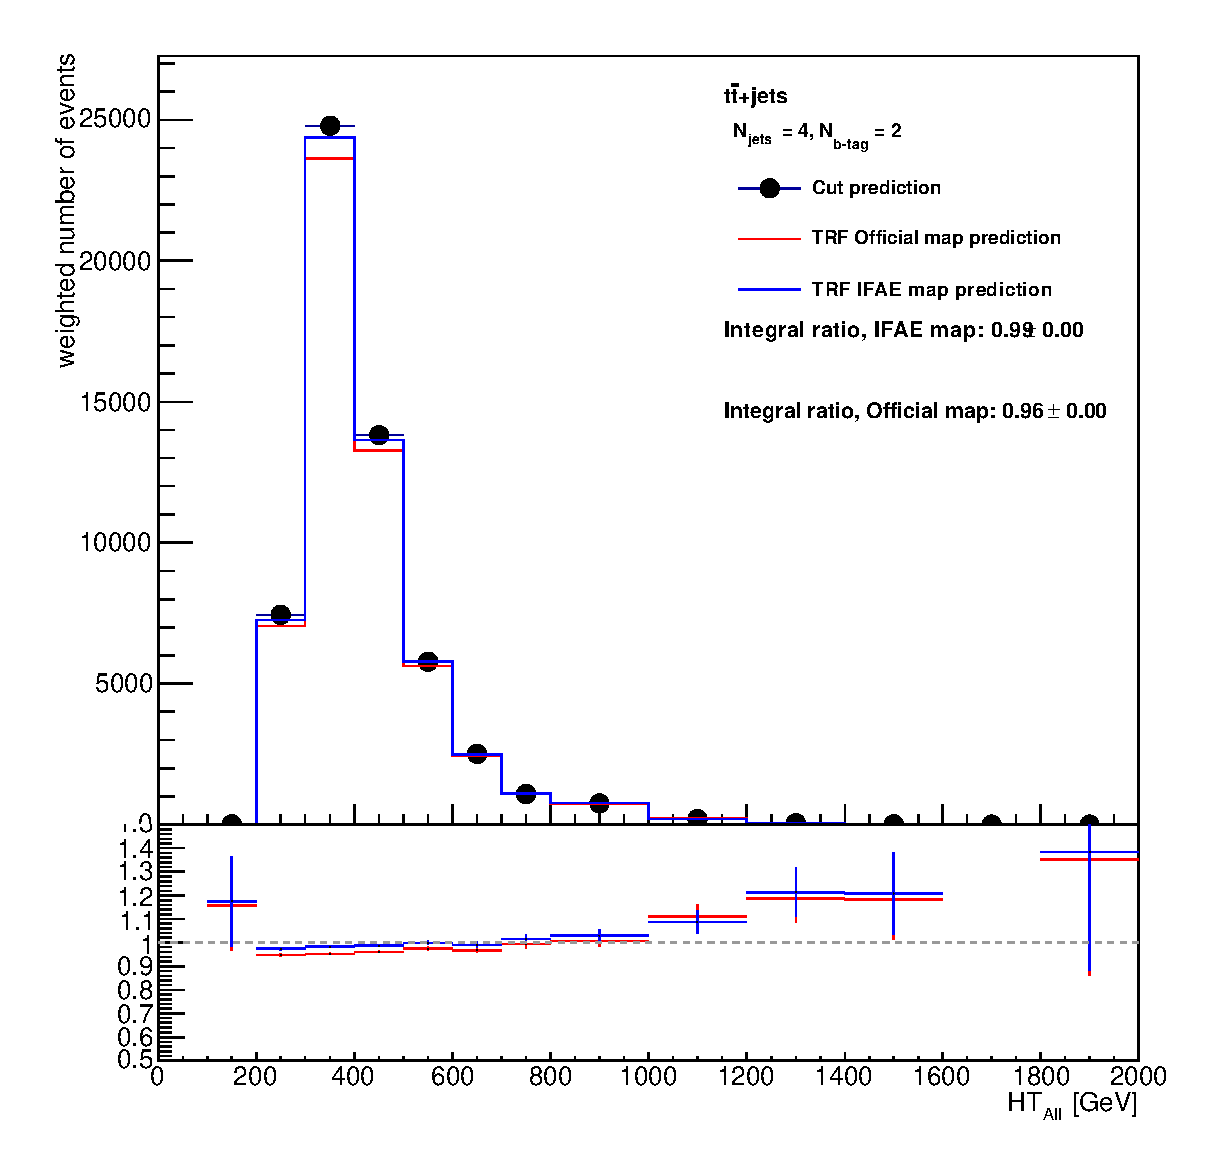
\includegraphics[width=0.3\textwidth]{appendices/figures/trf/ttbarAlpgen_HFOR_htall_4jetex2btagex.eps}}
	\subfigure[]{
  	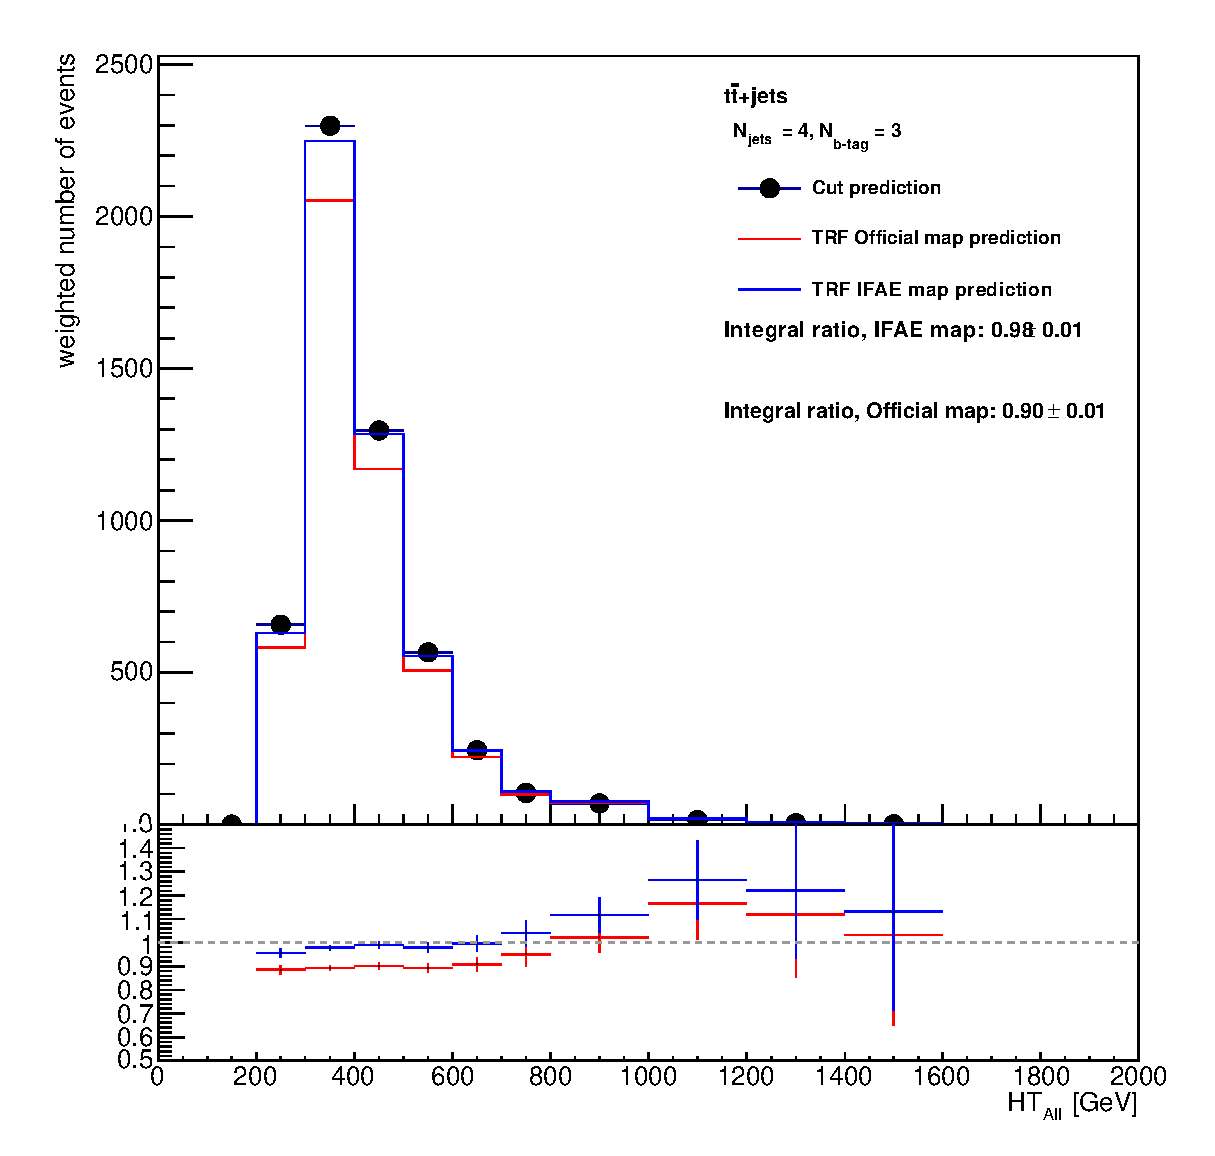
\includegraphics[width=0.3\textwidth]{appendices/figures/trf/ttbarAlpgen_HFOR_htall_4jetex3btagex.eps}}
	\subfigure[]{
  	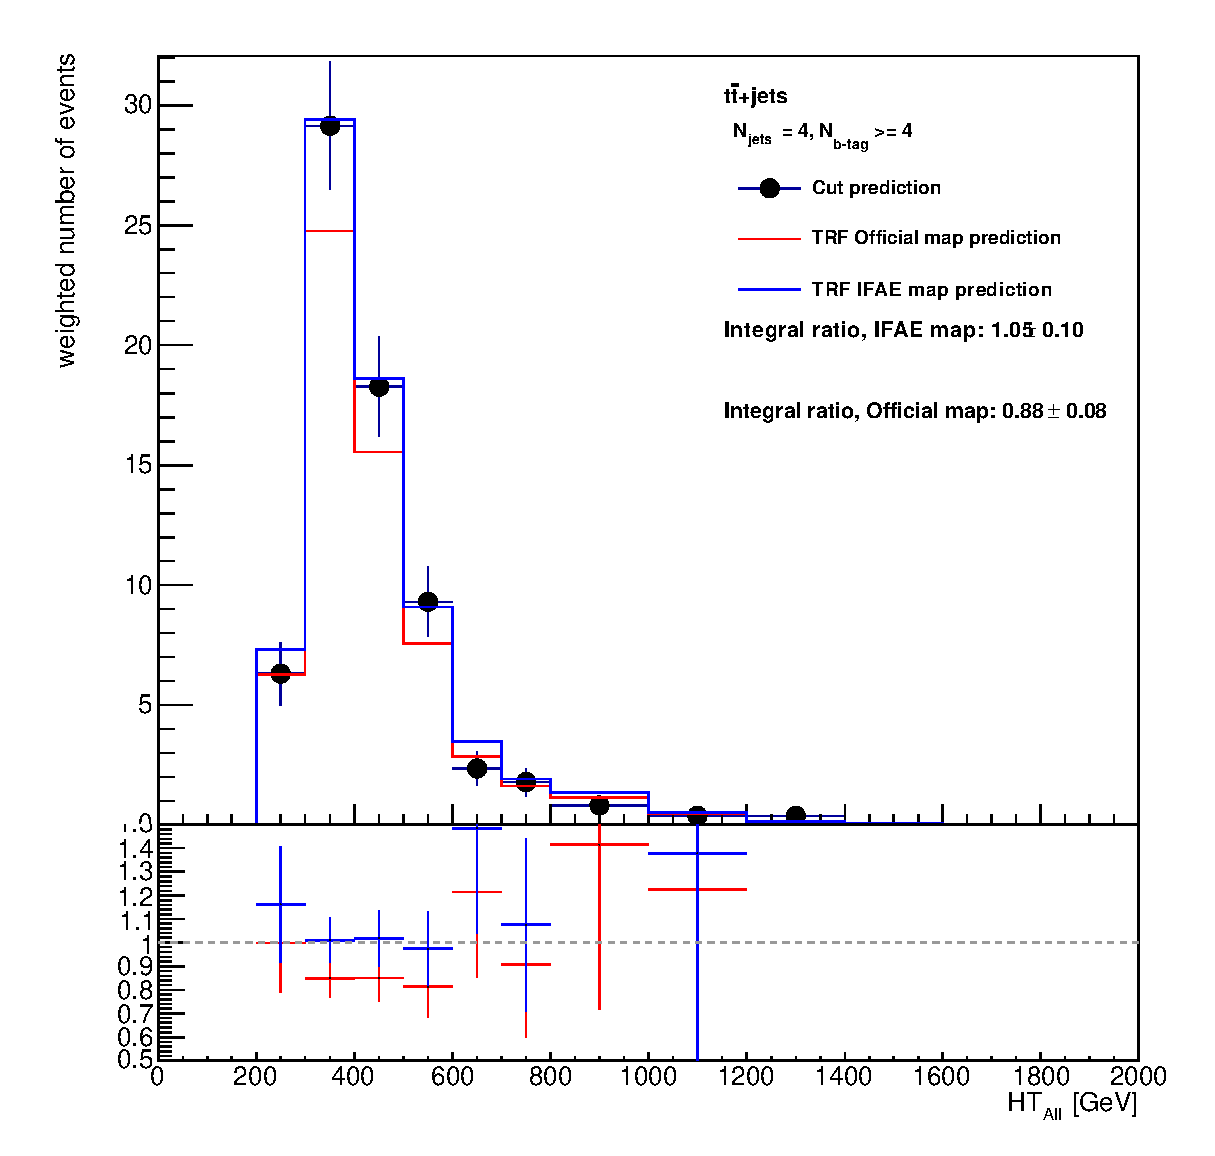
\includegraphics[width=0.3\textwidth]{appendices/figures/trf/ttbarAlpgen_HFOR_htall_4jetex4btagin.eps}}}\\
\hskip-1cm
\resizebox{1.5\textwidth}{!}{
	\subfigure[]{
  	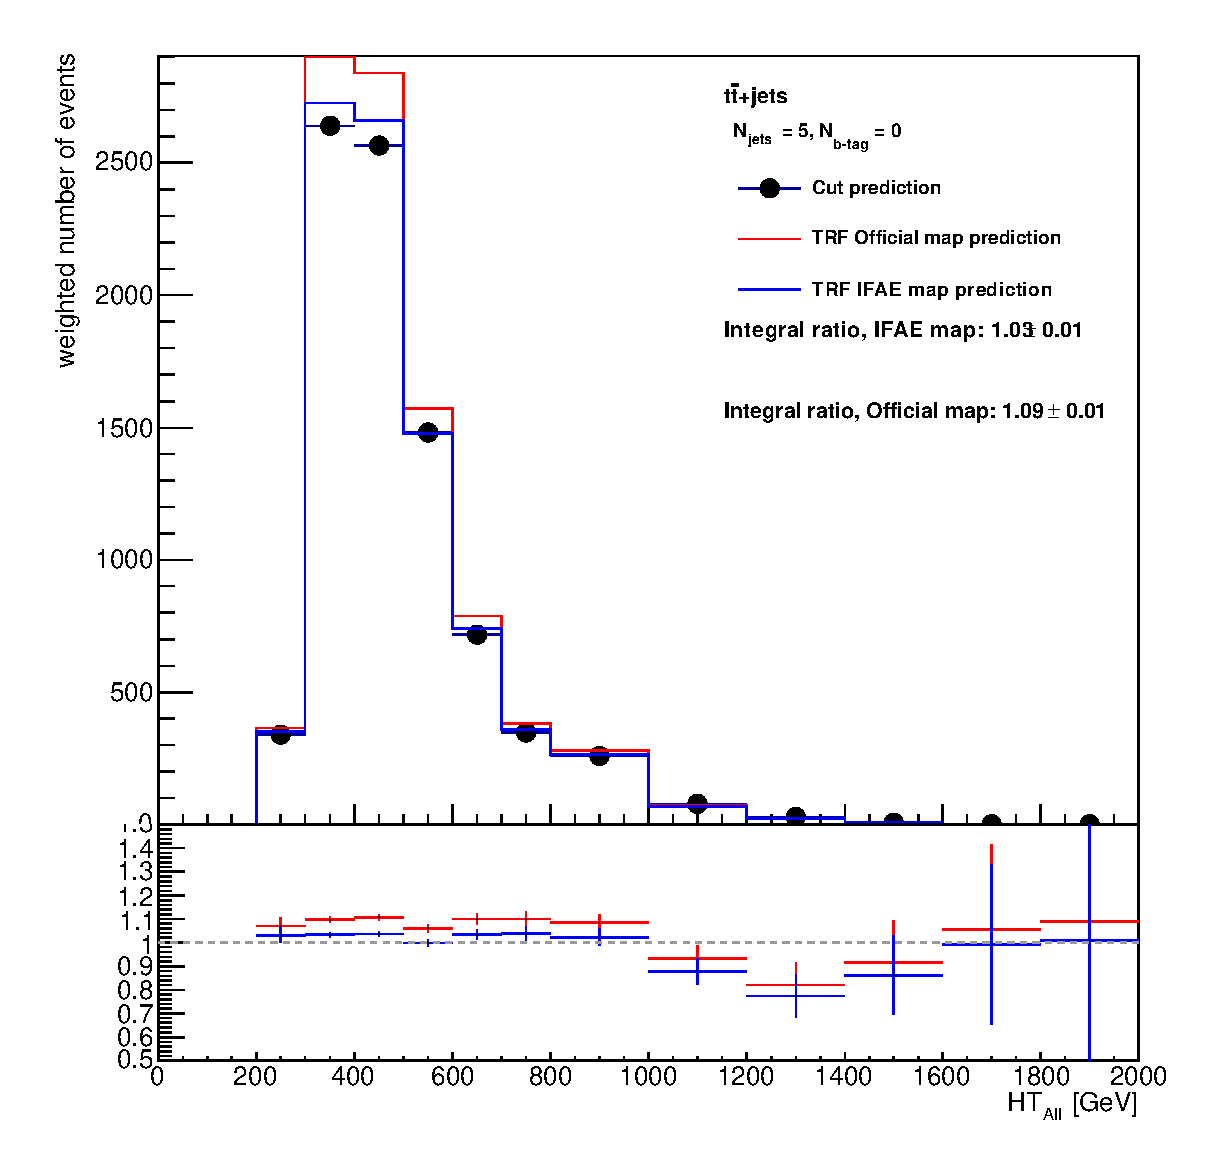
\includegraphics[width=0.3\textwidth]{appendices/figures/trf/ttbarAlpgen_HFOR_htall_5jetex0btagex.eps}}
	\subfigure[]{
  	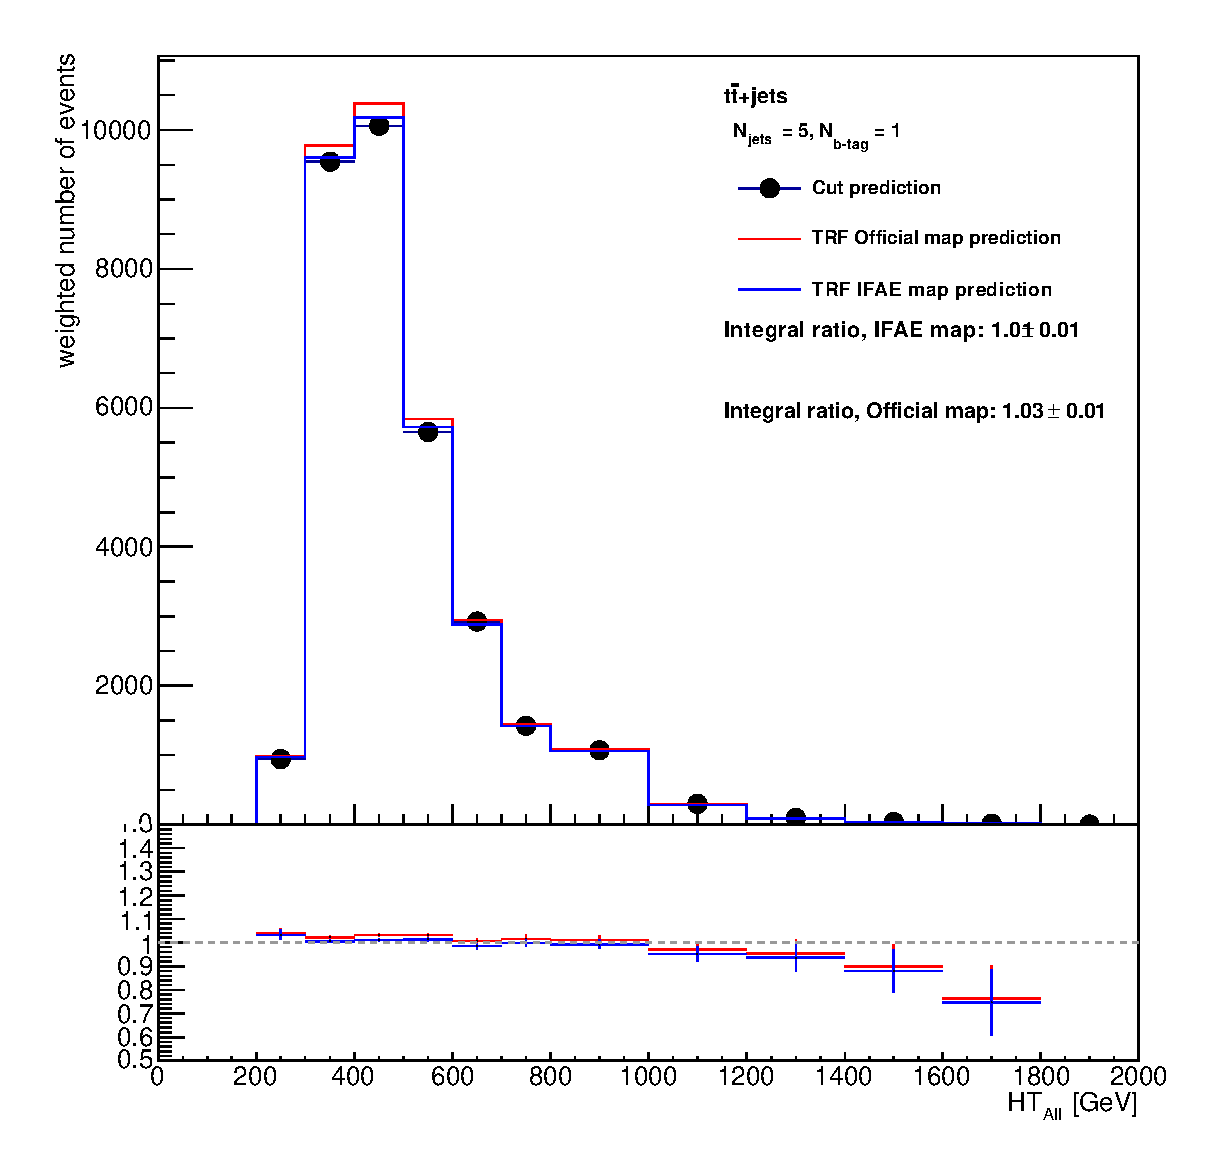
\includegraphics[width=0.3\textwidth]{appendices/figures/trf/ttbarAlpgen_HFOR_htall_5jetex1btagex.eps}}
	\subfigure[]{
  	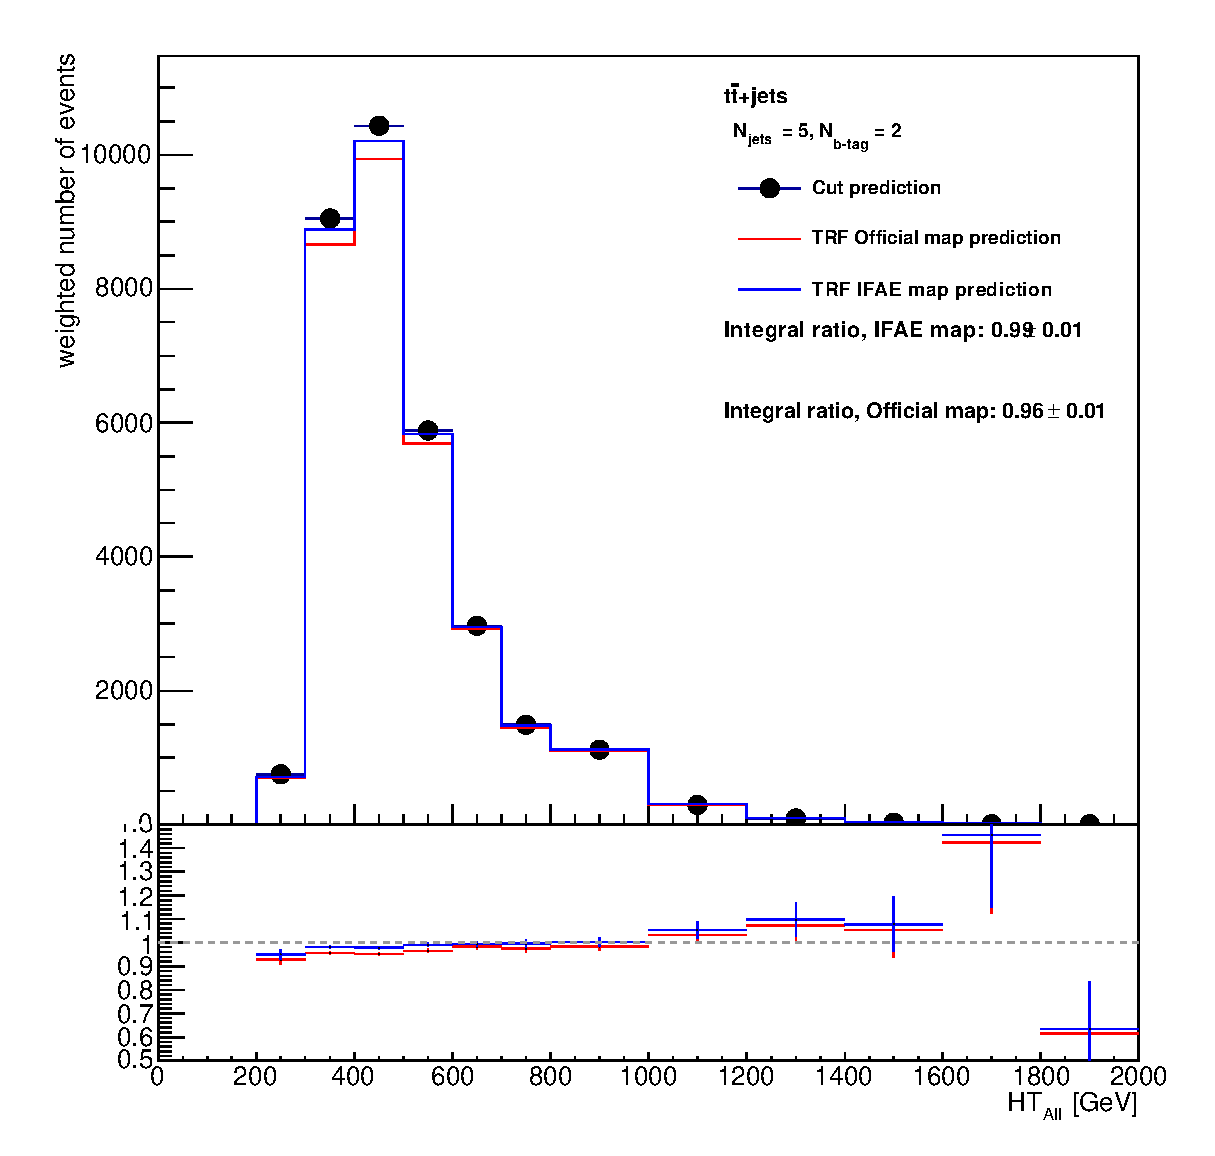
\includegraphics[width=0.3\textwidth]{appendices/figures/trf/ttbarAlpgen_HFOR_htall_5jetex2btagex.eps}}
	\subfigure[]{
  	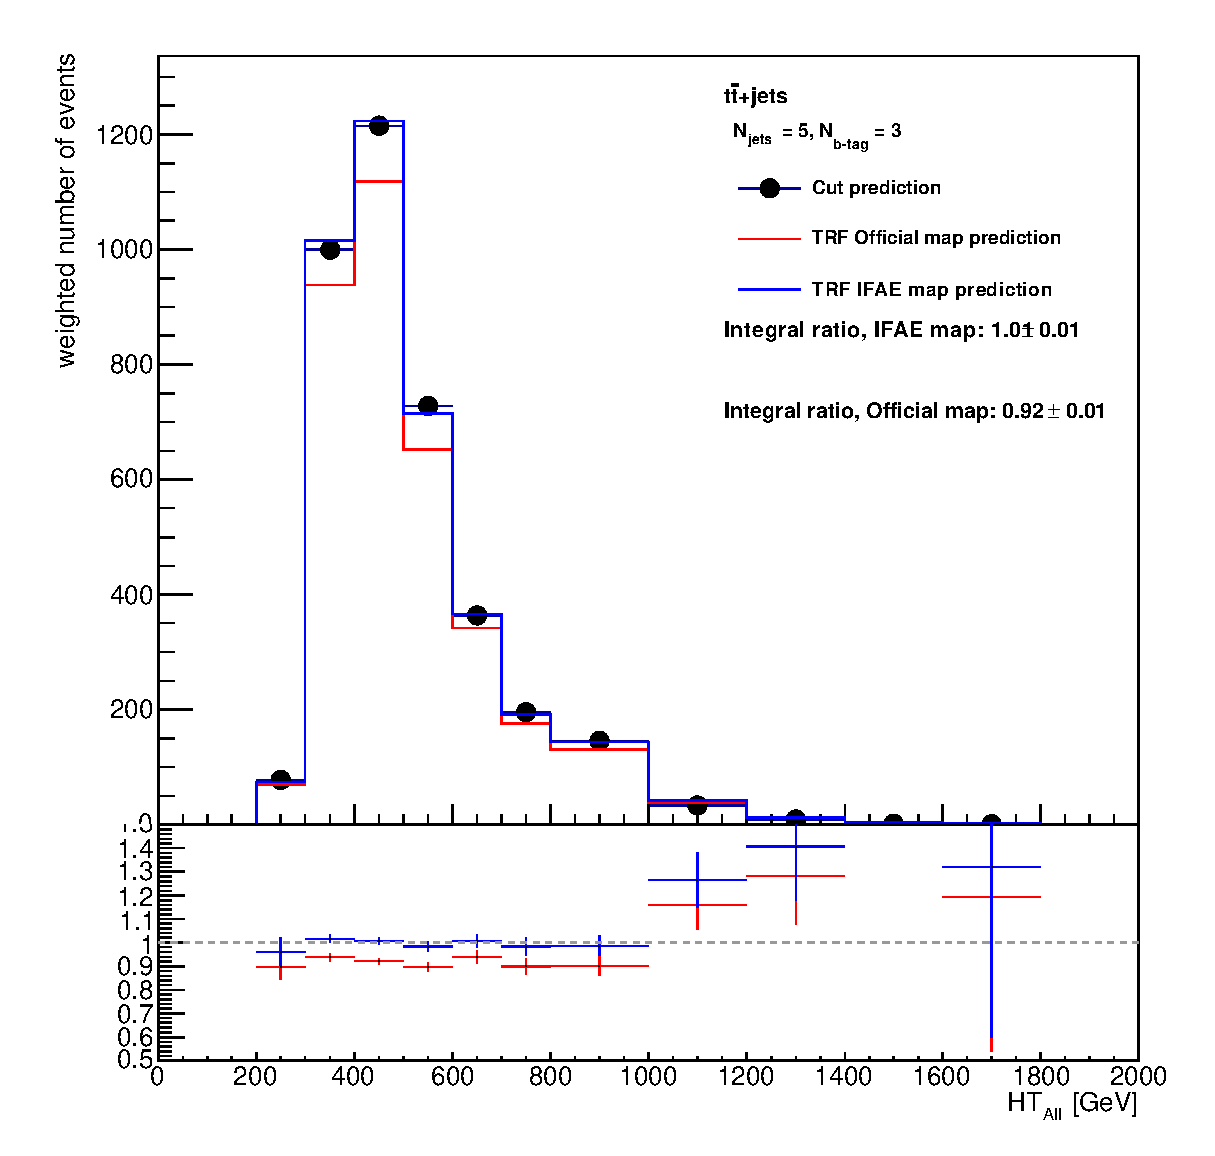
\includegraphics[width=0.3\textwidth]{appendices/figures/trf/ttbarAlpgen_HFOR_htall_5jetex3btagex.eps}}
	\subfigure[]{
  	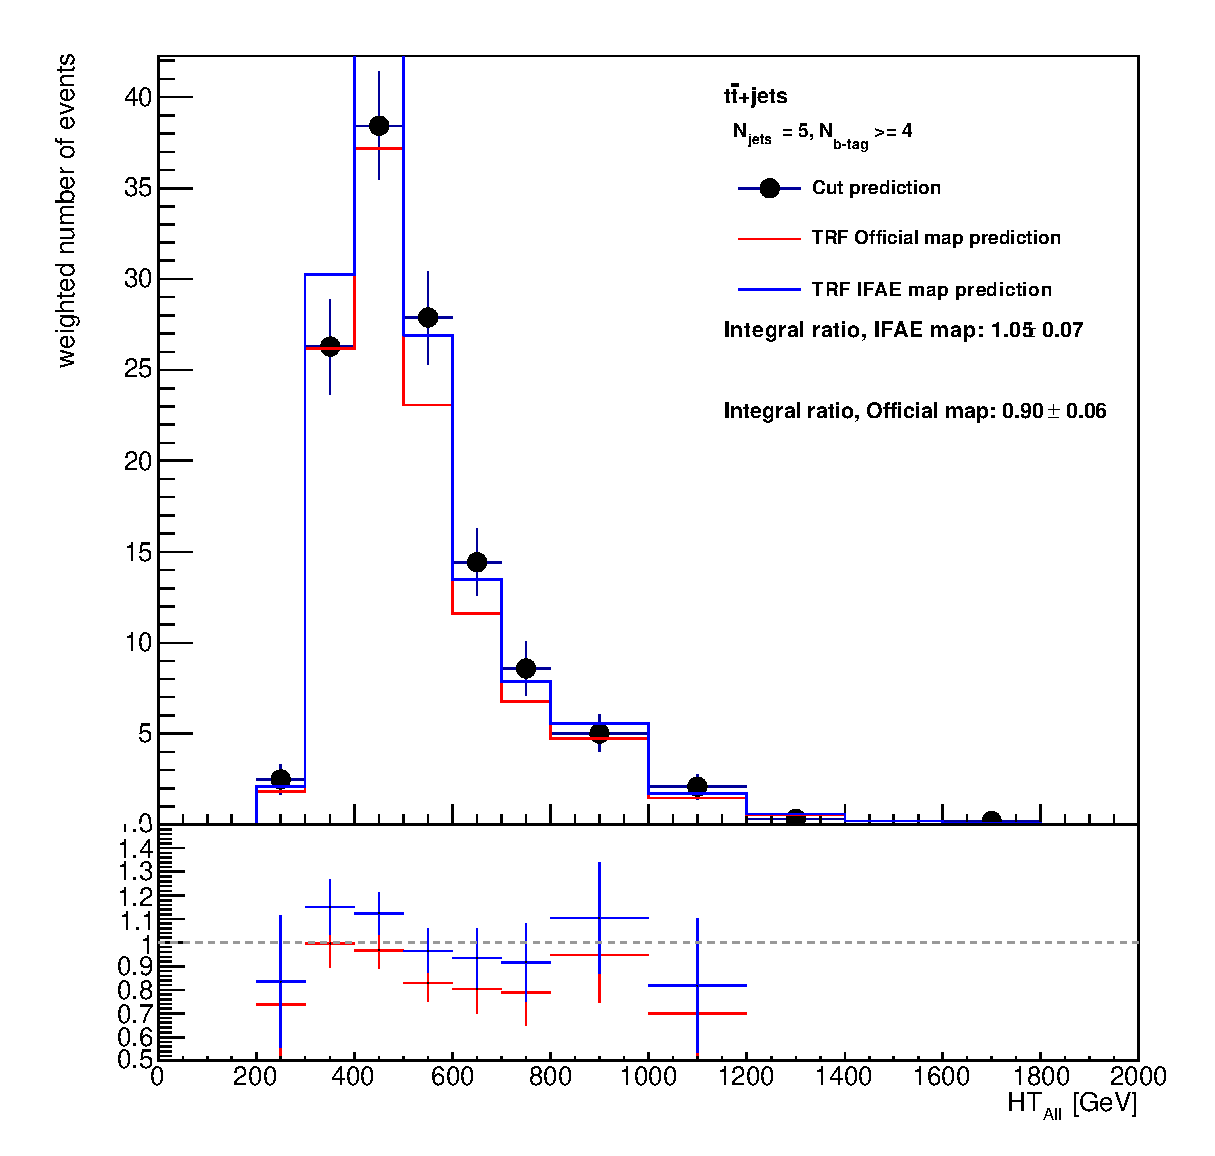
\includegraphics[width=0.3\textwidth]{appendices/figures/trf/ttbarAlpgen_HFOR_htall_5jetex4btagin.eps}}
}\\
\hskip-1cm
\resizebox{1.5\textwidth}{!}{
	\subfigure[]{
  	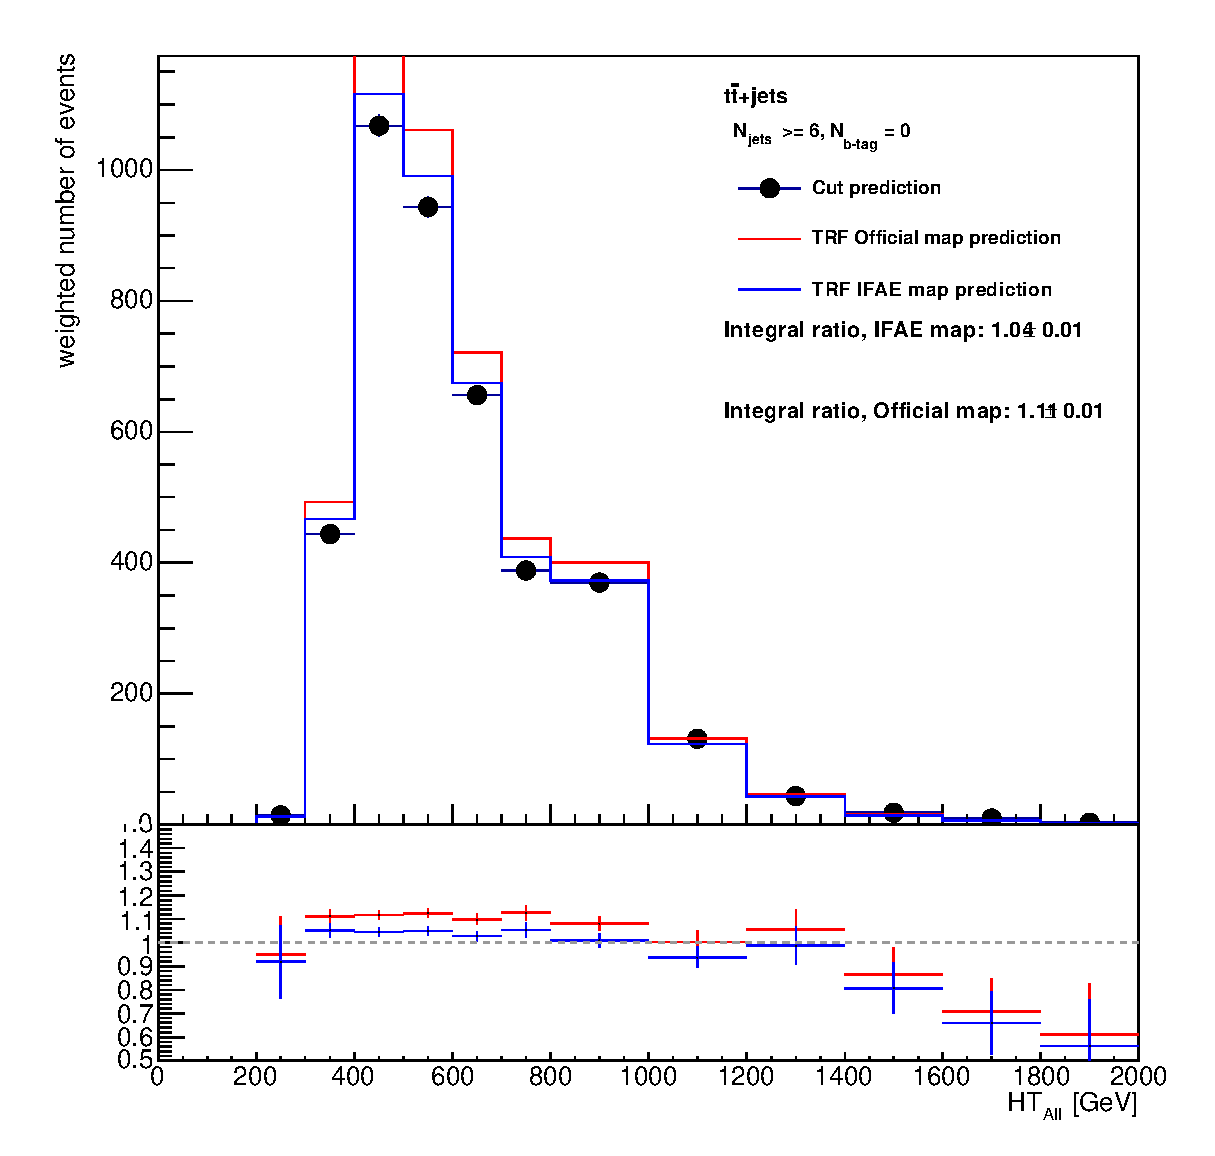
\includegraphics[width=0.3\textwidth]{appendices/figures/trf/ttbarAlpgen_HFOR_htall_6jetin0btagex.eps}}
	\subfigure[]{
  	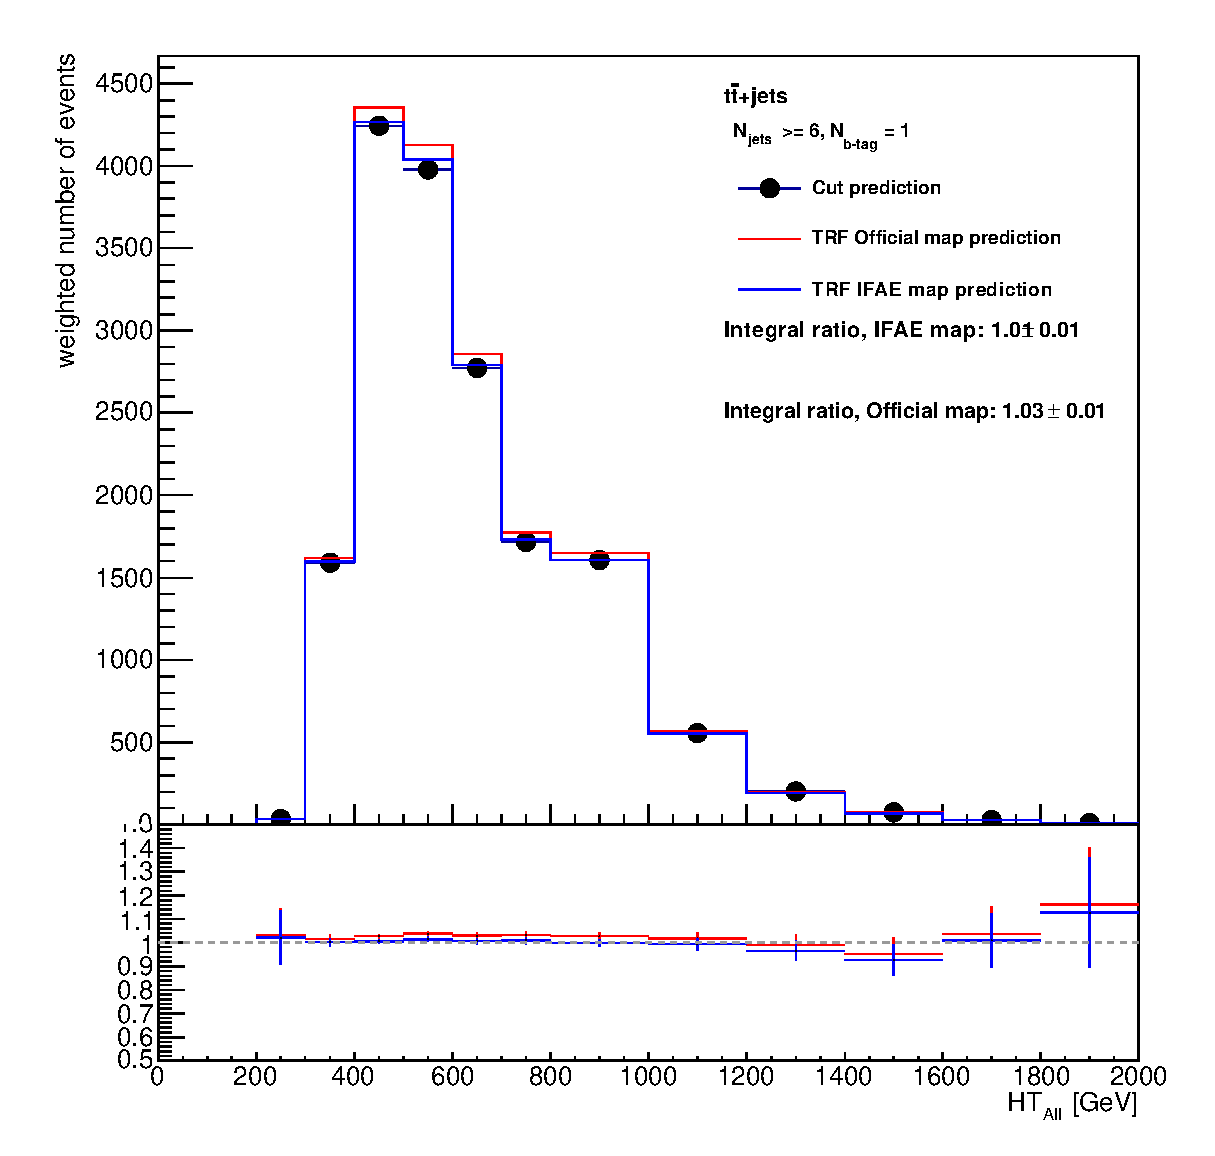
\includegraphics[width=0.3\textwidth]{appendices/figures/trf/ttbarAlpgen_HFOR_htall_6jetin1btagex.eps}}
	\subfigure[]{
  	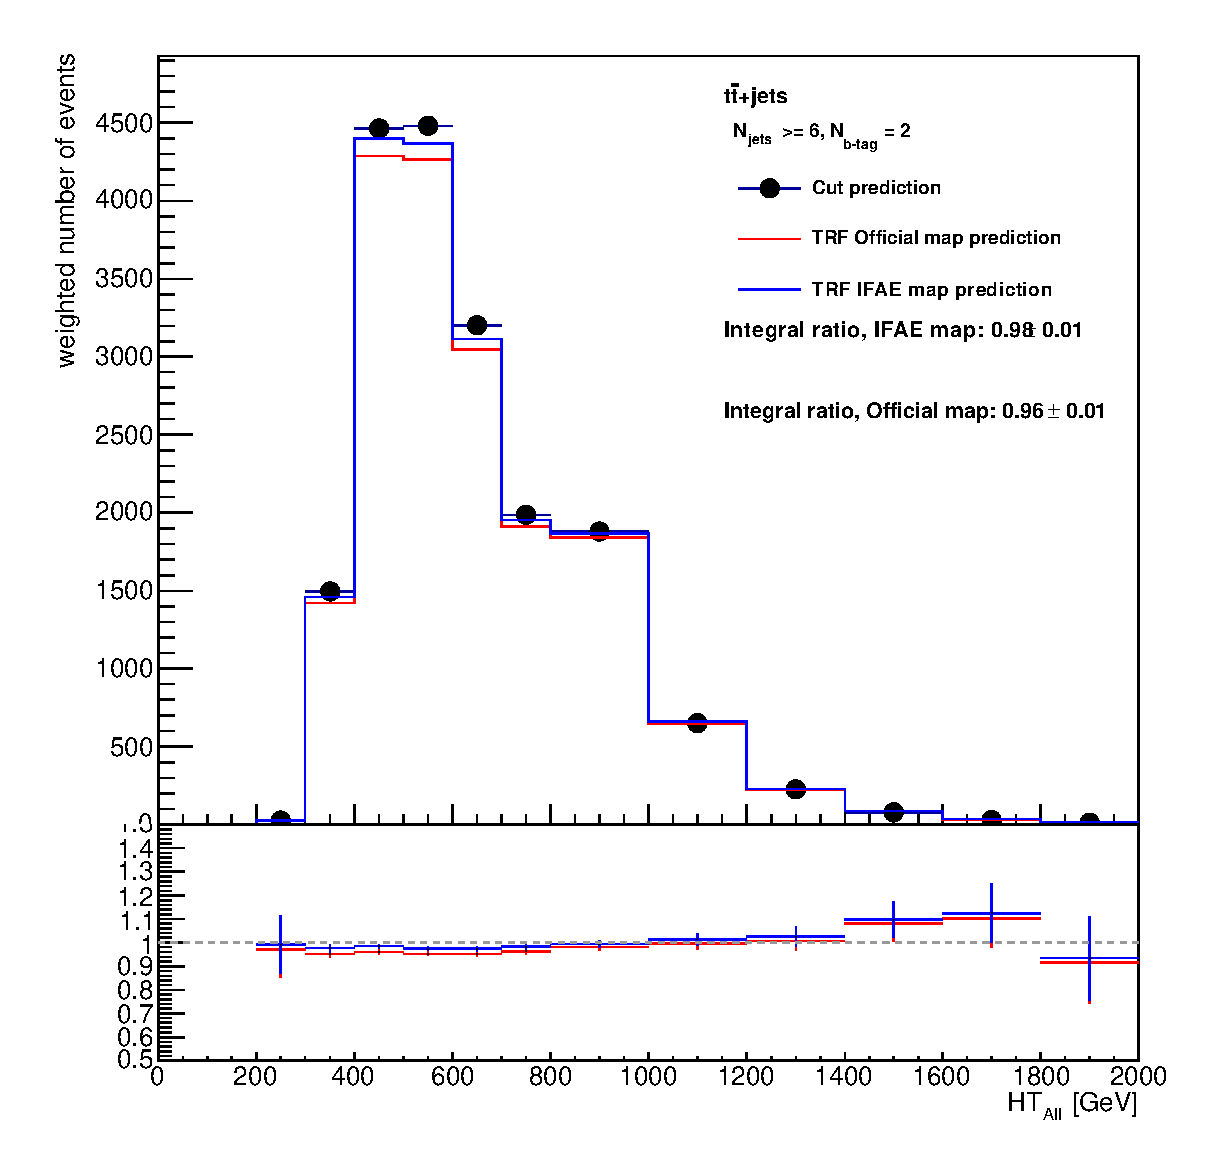
\includegraphics[width=0.3\textwidth]{appendices/figures/trf/ttbarAlpgen_HFOR_htall_6jetin2btagex.eps}}
	\subfigure[]{
  	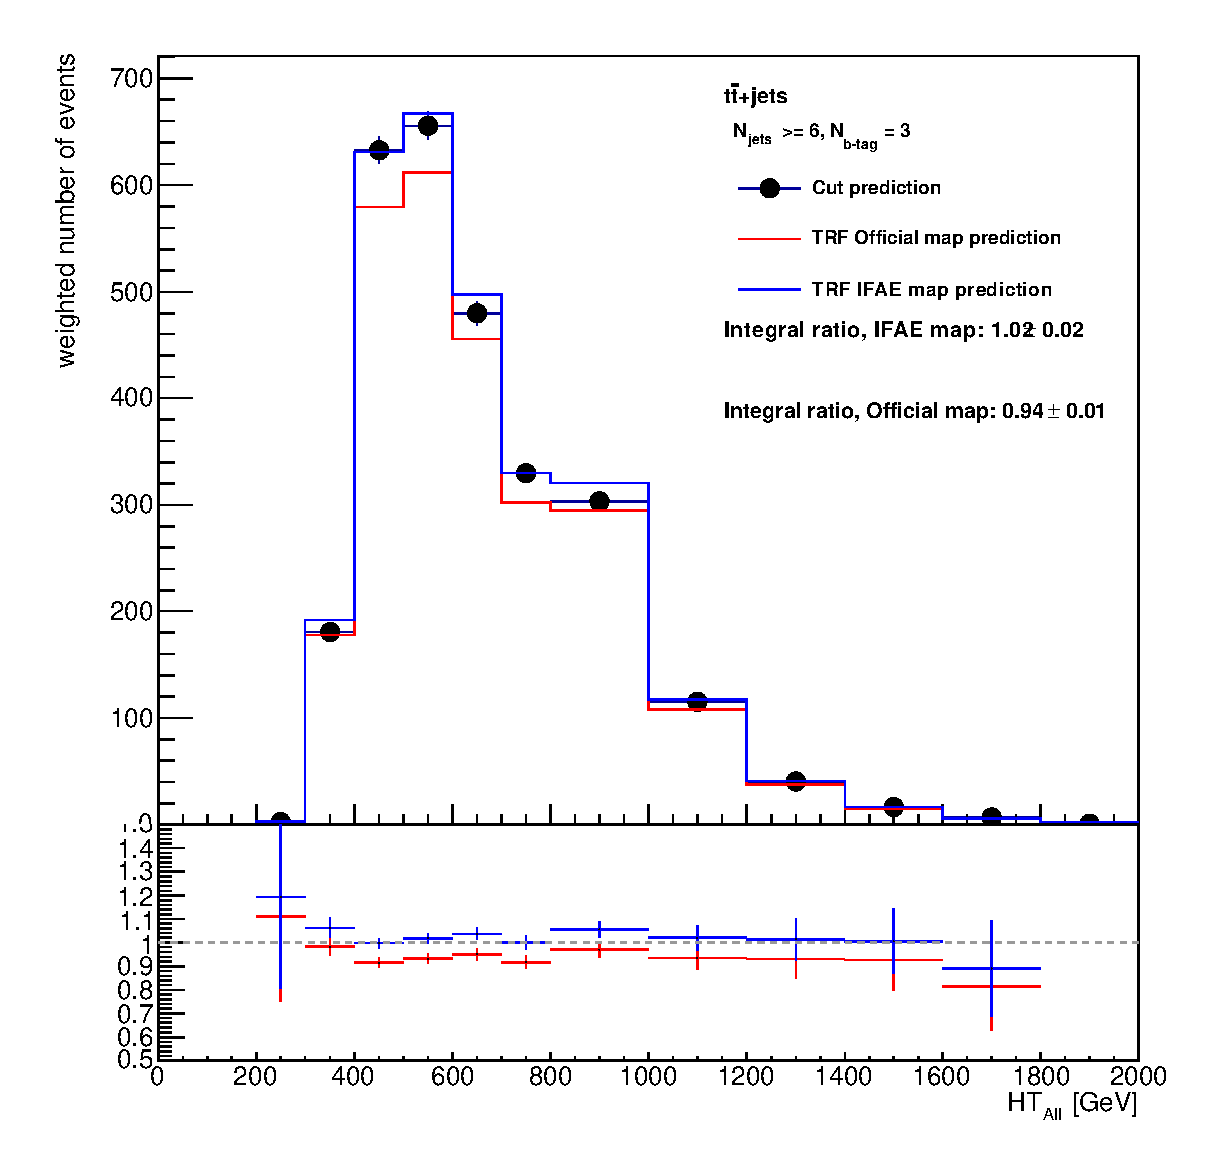
\includegraphics[width=0.3\textwidth]{appendices/figures/trf/ttbarAlpgen_HFOR_htall_6jetin3btagex.eps}}
	\subfigure[]{
  	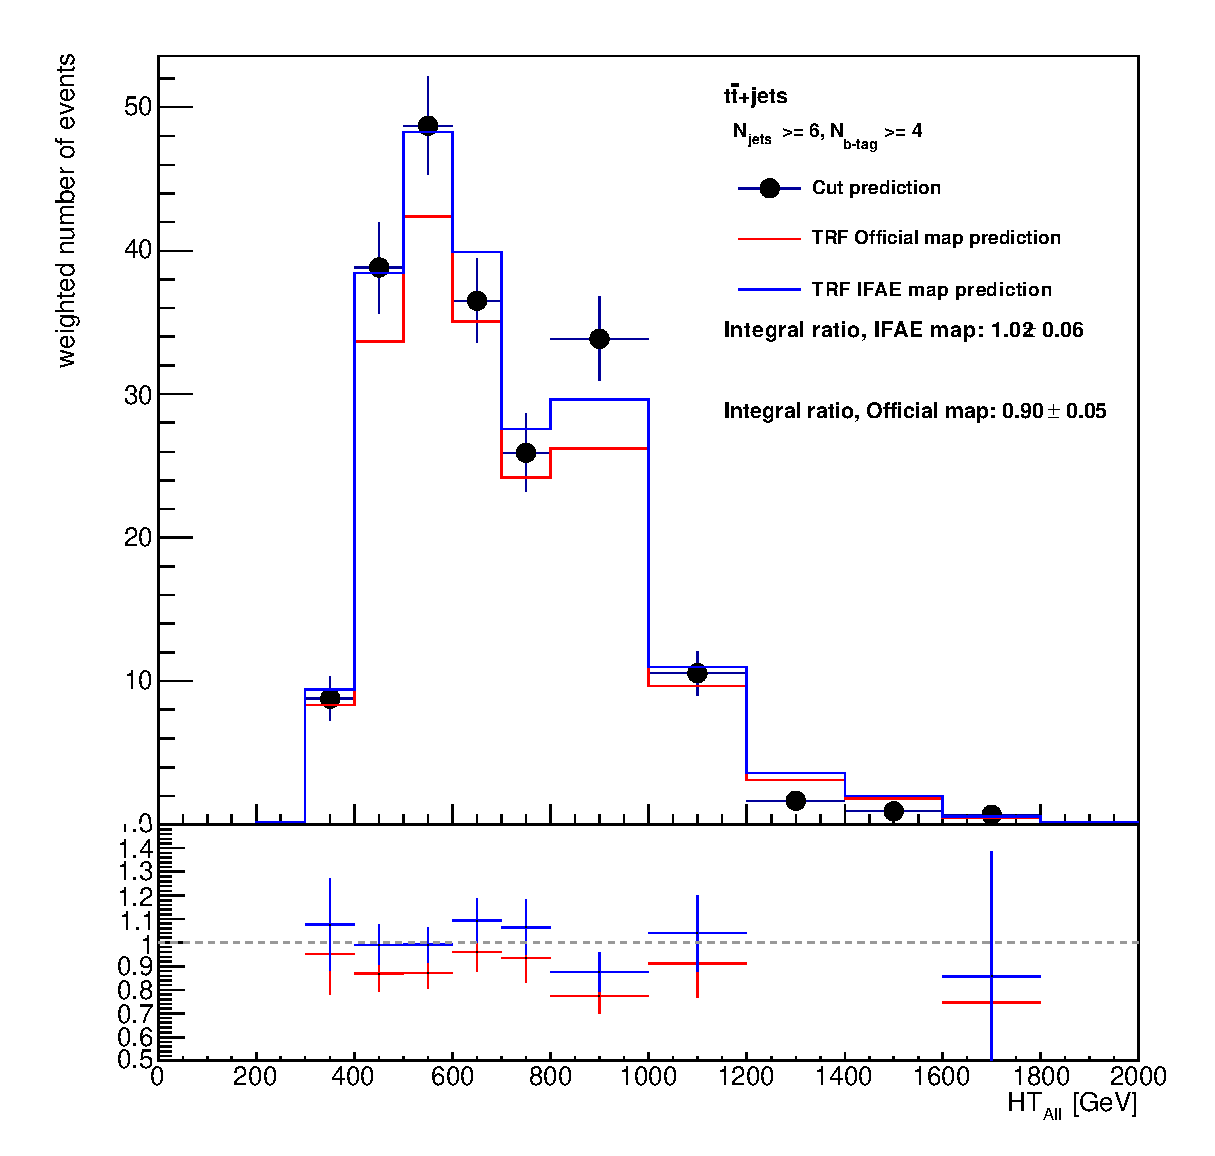
\includegraphics[width=0.3\textwidth]{appendices/figures/trf/ttbarAlpgen_HFOR_htall_6jetin4btagin.eps}}
}
	\caption{Comparison of the TRF and $b$-tag cut prediction for the $HT_{all}$ distribution in the (a--e) 4 jet exclusive, (f--j) 5 jet exclusive and (k--o) 6 jet inclusive channels, for different $b$-tagging multiplicities (from left to right, 0, 1, 2, 3 exclusive and 4 inclusive) for the $t\bar{t}$ \texttt{ALPGEN} sample. }
  \label{fig:validate_ttbar_ht}
\end{center}\end{figure}
\end{landscape}

%%%%%%%%%%%%%%%
\begin{table}\small
\begin{center}
\begin{tabular}{lcccc} \toprule
  & \multicolumn{2}{c}{TRF} & \multicolumn{2}{c}{Direct tagging}\\
  & Entries & Predicted yield & Entries & Predicted yield  \\
\midrule
\multicolumn{5}{c}{$W$+jets} \\
\midrule
Preselection            & 66381  & 37679.2 	$\pm$ 	324.0 	 & 8880  & 37317.3 	$\pm$ 	527.8 	\\
$\geq 1~W$              & 1321  & 723.2 	$\pm$ 	40.3 	 & 185  & 713.9 	$\pm$ 	66.7 	\\
$H_T>800~$GeV           & 520  & 314.0 	        $\pm$ 	27.4 	 & 84  & 308.0 	        $\pm$ 	41.7 	\\
$p_T(b_1) > 160~$GeV    & 262  & 146.9 	        $\pm$ 	17.8 	 & 44  & 155.3 	        $\pm$ 	30.5 	\\
$p_T(b_2) >80~$GeV      & 63  & 46.9 	        $\pm$ 	11.5 	 & 11  & 39.9 	        $\pm$ 	13.8 	\\
$\Delta R(l,\nu)<1.2$   & 28  & 16.3 	        $\pm$ 	6.0 	 & 5  & 14.7 	        $\pm$ 	7.2 	\\
min$\Delta R(l,b)>1.4$  & 15  & 6.3 	        $\pm$ 	2.8 	 & 2  & 5.2 	        $\pm$ 	4.0 	\\
min$\Delta R(W,b)>1.4$  & 9  & 5.5 	        $\pm$ 	2.8 	 & 1  & 3.7 	        $\pm$ 	3.7 	\\
\midrule
\multicolumn{5}{c}{$Z$+jets} \\
\midrule 
Preselection            & 19500  & 6054.4 	$\pm$ 	84.3 	 & 4573  & 6015.1 	$\pm$ 	147.7 	\\
$\geq 1~W$              & 331  & 133.9 	        $\pm$ 	14.2 	 & 87  & 125.9 	        $\pm$ 	19.0 	\\
$H_T>800~$GeV           & 130  & 47.8 	        $\pm$ 	8.7 	 & 32  & 49.4 	        $\pm$ 	12.2 	\\
$p_T(b_1) > 160~$GeV    & 74  & 25.2 	        $\pm$ 	6.7 	 & 19  & 29.8 	        $\pm$ 	10.2 	\\
$p_T(b_2) >80~$GeV      & 22  & 12.8 	        $\pm$ 	6.0 	 & 9  & 15.9 	        $\pm$ 	7.4 	\\
$\Delta R(l,\nu)<1.2$   & 5  & 1.1 	        $\pm$ 	0.6 	 & 1  & 0.8 	        $\pm$ 	0.8 	\\
min$\Delta R(l,b)>1.4$  & 2  & 0.2 	        $\pm$ 	0.2 	 & 0  & 0.0 	        $\pm$ 	0.0 	\\
min$\Delta R(W,b)>1.4$  & 2  & 0.2 	        $\pm$ 	0.2 	 & 0  & 0.0 	        $\pm$ 	0.0 	\\
\midrule
\multicolumn{5}{c}{Dibosons} \\
\midrule 
Preselection            & 18629  & 555.5 	$\pm$ 	7.0 	 & 3532  & 552.2 	$\pm$ 	11.4 	\\
$\geq 1~W$              & 336  & 10.9 	        $\pm$ 	1.1 	 & 50  & 8.6 	        $\pm$ 	1.4 	\\
$H_T>800~$GeV           & 85  & 2.9 	        $\pm$ 	0.6 	 & 14  & 2.4 	        $\pm$ 	0.7 	\\
$p_T(b_1) > 160~$GeV    & 32  & 0.9 	        $\pm$ 	0.3 	 & 4  & 0.5 	        $\pm$ 	0.3 	\\
$p_T(b_2) >80~$GeV      & 14  & 0.5 	        $\pm$ 	0.2 	 & 2  & 0.3 	        $\pm$ 	0.2 	\\
$\Delta R(l,\nu)<1.2$   & 9  & 0.2 	        $\pm$ 	0.1 	 & 1  & 0.1 	        $\pm$ 	0.1 	\\
min$\Delta R(l,b)>1.4$  & 8  & 0.1 	        $\pm$ 	0.1 	 & 1  & 0.1 	        $\pm$ 	0.1 	\\
min$\Delta R(W,b)>1.4$  & 4  & 0.1 	        $\pm$ 	0.0 	 & 0  & 0.0 	        $\pm$ 	0.0 	\\
\midrule
\multicolumn{5}{c}{Single top} \\
\midrule 
Preselection            & 74327  & 14670.8 	$\pm$ 	97.9 	 & 59854  & 14722.9 	$\pm$ 	107.0 	\\
$\geq 1~W$              & 2799  & 469.9 	$\pm$ 	14.1 	 & 2349  & 468.0 	$\pm$ 	14.9 	\\
$H_T>800~$GeV           & 986  & 164.7 	        $\pm$ 	7.9 	 & 826  & 162.8 	$\pm$ 	8.4 	\\
$p_T(b_1) > 160~$GeV    & 624  & 105.2 	        $\pm$ 	6.4 	 & 539  & 107.6 	$\pm$ 	6.9 	\\
$p_T(b_2) >80~$GeV      & 292  & 51.6 	        $\pm$ 	4.4 	 & 263  & 53.8 	        $\pm$ 	4.7 	\\
$\Delta R(l,\nu)<1.2$   & 165  & 30.2 	        $\pm$ 	3.6 	 & 147  & 30.4 	        $\pm$ 	3.7 	\\
min$\Delta R(l,b)>1.4$  & 61  & 14.0 	        $\pm$ 	2.4 	 & 55  & 14.0 	        $\pm$ 	2.4 	\\
min$\Delta R(W,b)>1.4$  & 21  & 4.4 	        $\pm$ 	1.3 	 & 19  & 4.8 	        $\pm$ 	1.4 	\\
\midrule
\multicolumn{5}{c}{$t\bar{t}V$} \\
\midrule 
Preselection            & 171489  & 706.1 	$\pm$ 	2.1 	 & 142296  & 709.0 	$\pm$ 	2.3 	\\
$\geq 1~W$              & 19492  & 78.6 	$\pm$ 	0.7 	 & 15862  & 78.3 	$\pm$ 	0.8 	\\
$H_T>800~$GeV           & 8516  & 34.2 	        $\pm$ 	0.5 	 & 6963  & 34.2 	$\pm$ 	0.5 	\\
$p_T(b_1) > 160~$GeV    & 4419  & 17.9 	        $\pm$ 	0.3 	 & 3657  & 18.0 	$\pm$ 	0.4 	\\
$p_T(b_2) >80~$GeV      & 2267  & 9.3        	$\pm$ 	0.2 	 & 1912  & 9.5 	        $\pm$ 	0.3 	\\
$\Delta R(l,\nu)<1.2$   & 1227  & 5.1 	        $\pm$ 	0.2 	 & 1029  & 5.2 	        $\pm$ 	0.2 	\\
min$\Delta R(l,b)>1.4$  & 321  & 1.3 	        $\pm$ 	0.1 	 & 265  & 1.4 	        $\pm$ 	0.1 	\\
min$\Delta R(W,b)>1.4$  & 138  & 0.5 	        $\pm$ 	0.1 	 & 104  & 0.6 	        $\pm$ 	0.1 	\\
\bottomrule
\end{tabular}
    
\caption{Comparison of expected yields between TRF and direct tagging as a function of cuts applied from the preselection level up to the \tight\ selection.\label{tab:TRFvsCUT}}
\end{center}
\end{table}
%%%%%%%%%%%%%%%
